\chapter{The Mercury I/O Middleware}
In this chapter we present the Mercury middleware design and implementation. The main goal of Mercury is to provide users with a simple interface that allows to express I/O pattern. This knowledge is used by the middleware
to optimize data access through data prefetching. In particular Mercury exploits the concept of data sieving. Data sieving can improve performance when the application is reading non contiguously data from a limited region
of the block device. In this case all the region is brought into main memory and non-contiguous accesses can thus be served from the fast RAM. At this point the cache also contains data that is not required thus wasting
space. Nevertheless, if data sieving is performed properly the data can be evicted from the cache and memory wasting can be kept to the minimum. This is done by Mercury in a transparent way to the user.

\section{Introduction}
\label{sec: motivation}
As already said in the introduction, the I/O performance gap problem represents a serious scalability limitation for scientific applications running on HPC clusters. Parallel File Systems such as Lustre and GPFS try to bridge this gap by striping 
files across multiple storage devices and providing multiple parallel data paths to increase the aggregate I/O bandwidth and the number of I/O Operations per Second (IOPS). The ROMIO middleware implements extensions to the POSIX I/O interface typically 
provided by PFSs that result in a richer parallel I/O interface, and through the ADIO drivers enables transparent file access optimizations based on two-phase I/O and data sieving to adapt I/O patterns to the characteristics of the underlying file 
system~\cite{ThakurGL99}~\cite{Ying08}~\cite{ProstTHKW00}.

Nevertheless, as Carns et al. have pointed out in their study~\cite{CarnsHABLLR11} most of the scientific applications running on big clusters today still use the POSIX I/O interface to access their data. Furthermore, it has also been ascertained 
that using POSIX I/O to access non-contiguous regions of the file causes extremely poor performance in the case of PFSs~\cite{ChingCLP06}. Indeed, PFSs provide best I/O bandwidth performance for large contiguous requests while they typically provide 
only a fraction of the maximum bandwidth in the opposite case. This is primarily due to the high number of remote procedure calls generated by the file system clients that overwhelms I/O servers, the resulting high number of HDDs' head movements in 
every I/O target (seek overhead) and ultimately by the file system block locking contention.

Currently there is no available solution to overcome limitations caused by non-optimal file I/O patterns generated by applications, except to re-write them. In this context, the Linux kernel provides users with the capability to communicate access 
pattern information to the local file system through the \texttt{posix\_fadvise()}~\cite{AdviseAPI} system call. The file system can use this information to improve page cache efficiency, for example, by prefetching (or releasing) data that will 
(or will not) be required soon in the future or by disabling read-ahead in the case of random read patterns. However, \texttt{posix\_fadvise()} is barely used in practice and has intrinsic limitations that discourage its employment in real applications.

The two most used PFSs in HPC clusters nowadays, IBM GPFS and Lustre, are both POSIX compliant. However, neither of them support the POSIX advice mechanism previously described. GPFS compensates for the lack of POSIX advice support through a hints API 
that users can access by linking their programs against a service library. Hints are passed to GPFS through the \texttt{gpfs\_fcntl()}~\cite{GPFSHINTS} function and can be used to guide prefetching (or releasing) of file blocks in the page pool
\footnote{GPFS pinned memory used for file system caching.}. However, unlike POSIX advice, GPFS hints can be discarded by the file system if certain requirements are not met. Lustre, on the other hand, does not provide any client side mechanism similar 
to GPFS hints or POSIX advice. A new Lustre advice mechanism has been proposed by DDN during the Lustre User Group 2014 (LUG14) in Miami~\cite{Comer14}. The DDN approach provides control over the storage servers (OSSs) cache instead of the file 
system client cache.

In this thesis we propose and evaluate a novel guided I/O framework called \textit{Mercury}~\cite{mercury} able to optimize file access patterns at run-time through data prefetching using available hints mechanisms. Mercury communicates file I/O pattern 
information to the file system on behalf of running applications using a dedicated process that we call \textit{Advice Manager}. In every node of the cluster, processes can access their files using an \textit{Assisted I/O library} that transparently 
forwards intercepted requests to the local \textit{Advice Manager}. This uses \texttt{posix\_fadvise()} and \texttt{gpfs\_fcntl()} to prefetch (or release) data into (or from) the client's file system data cache. The \textit{Assisted I/O library} controls 
for which files advice or hints should be given, while the \textit{Advice Manager} controls how much data to prefetch (or release) from each file. Monitored file paths and prefetching information are contained in a configuration file that can be generated 
either manually or automatically once the I/O behaviour of the target application is known. The configuration file mechanism allows us to decouple the specific hints API provided by the back-end file system from the generic interface exposed to the final 
user thus making our solution portable.

With this approach we are able to generate POSIX advice and GPFS hints for applications that do not use them but can receive a benefit from their use. We accomplish this asynchronously and without any modification of the original application. We demonstrate 
that our approach is effective in improving the I/O bandwidth, reducing the number of I/O requests and reducing the execution time of a `ROOT' \footnote{Data analysis framework developed at CERN.}~\cite{root} based analytic application.

Additionally, we propose and evaluate a modification to the Linux kernel that makes it possible for Lustre, and in principle other networked file systems, to participate in activity triggered by the \texttt{posix\_fadvise()} system call, thus allowing it to 
take advantage of our guided I/O framework benefits.

The remainder of this chapter is organised as follows. Section~\ref{sec: mercury_concept} presents concept, design and implementation of the MERCURY prototype highlighting the main contributions of the work. This section also describes the kernel modifications 
that enable POSIX advice on Lustre, Section~\ref{sec: mercury_evaluation} presents the evaluation of our prototype on three file systems: a local Linux ext4 file system, a GPFS file system and a Lustre file system, Section~\ref{sec: mercury_related_work} presents 
related works on data prefetching, and finally Section~\ref{sec: mercury_conclusion} presents conclusion and future work.

\section{Mercury Concept \& Design}
\label{sec: mercury_concept}
The first part of this section presents the concept, design and the implementation of the Mercury prototype. The second part describes the Linux kernel modifications that allow Lustre to work with our solution through the posix\_fadvise interface.

The I/O software stack of Mercury is depicted in Figure~\ref{figure: softwarestack}. Besides the standard I/O libraries we add two software components, an \textit{Assisted I/O library} (AIO), used to intercept I/O calls issued by applications and an 
\textit{Advice Manager} (AM) process that receives messages sent from the \textit{Assisted I/O library} and generates POSIX advice and GPFS hints. The library is preloaded by the runtime linker before other libraries through the \texttt{LD\_PRELOAD} 
mechanism and uses UNIX domain sockets to communicate with the \textit{Advice Manager}. In the case of GPFS hints \textit{libgpfs} provides the correct hints API to the \textit{Advice Manager}, other file systems will use the posix\_fadvise syscall.

\begin{figure}[!htb]
  \centering
  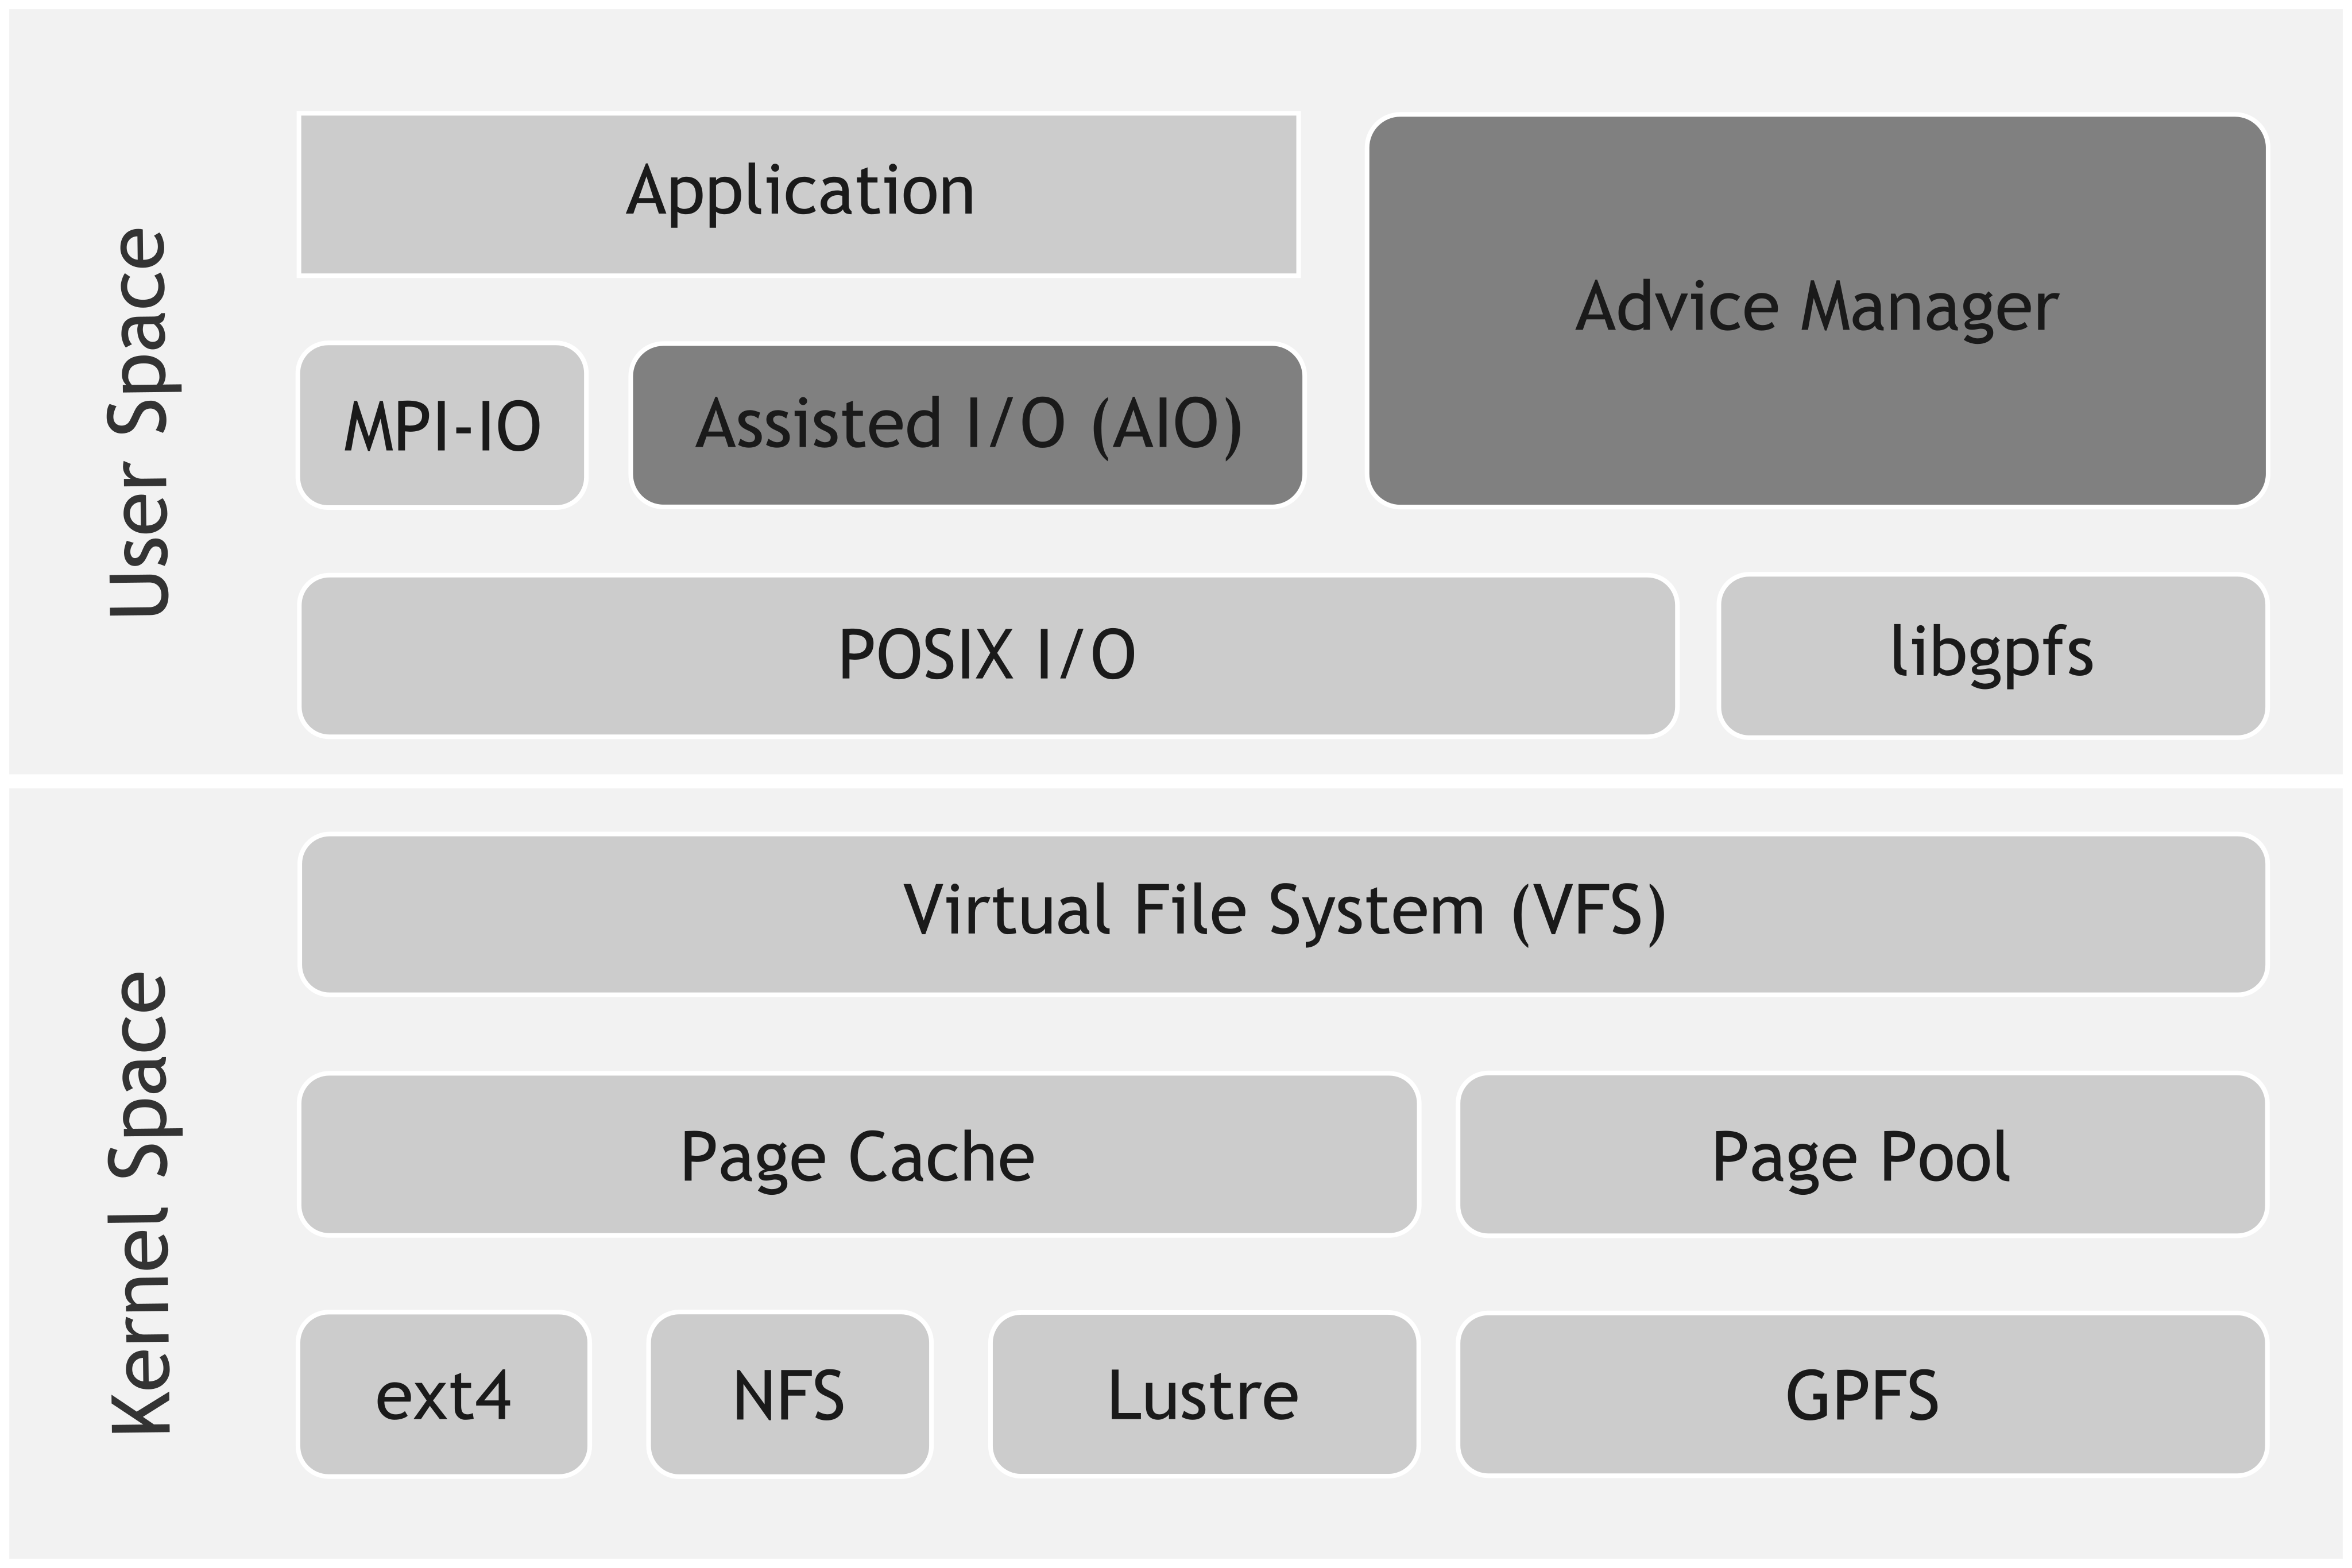
\includegraphics[width=0.8\textwidth]{chapters/chapter2/figures/linux-software-stack-ext}
  \caption{Mercury I/O software stack. \textit{Assisted I/O library} and \textit{Advice Manager} communicate through UNIX domain sockets. The AM binds its socket to the local file system pathname \texttt{/tmp/channel}, while the AIO connects its socket 
  to the same pathname; exactly in the same way they would bind and connect to an IP address if they were located on different nodes in the network. Unix domain sockets are used to pass ancillary data as well as custom messages between the two software 
  entities. Data can reside in a local Linux file system, in Lustre or in GPFS.}
  \label{figure: softwarestack}
\end{figure}

The proposed architecture adds two major contributions. First of all, it allows us to use the Linux advice API as well as the GPFS hints API asynchronously through the \textit{Advice Manager}. This means that we can effectively overlap I/O and computation 
phases in target applications. Secondly, it enables us to generate POSIX advice and GPFS hints transparently, without the need to modify the application. The information required by the \textit{Advice Manager} is extracted from observations of the application's 
I/O behaviour~\footnote{How this can be done effectivelly and in a generalized way is itself a research topic and is therefore left as part of future works.} during a set of preliminary runs and then written to a configuration file to be used in following runs.

In the rest of this section we describe the different aspects of our design including the interprocess communication between the two software entities and the prefetching request generation using the \texttt{posix\_fadvise()} system call or the 
\texttt{gpfs\_fcntl()} function.

\subsection{Interprocess Communication}
\label{subsec: interprocess_comm}
We now describe how interprocess communication is implemented and how messages sent from the \textit{Assisted I/O library} are handled by the \textit{Advice Manager}. Figure~\ref{figure: architecture} depicts the architecture of the two software components 
introduced by our design. The \textit{Advice Manager} is made up of three smaller modules: a \textit{Request Manager} (RM) that receives requests sent by the \textit{Assisted I/O library}, a \textit{Register Log} (RL) that keeps track of which files are 
currently handled by the \textit{Advice Manager}, and an \textit{Advisor Thread} (AT) that receives read requests from the \textit{Request Manager} through a queue and issues POSIX advice and GPFS hints.

In order to enable asynchronous prefetching we delegate the task of sending synchronous hints or advice to the \textit{Advice Manager}. When an application issues an open call for a file, the \textit{Assisted I/O library} intercepts it, performs the open and 
then sends a message to the \textit{Advice Manager}. The message contains a string of the form: \texttt{"\textbf{Register} \textit{pid} \textit{pathname} \textit{fd}"}, plus additional ancillary information explained later. This string tells the \textit{Request 
Manager} to register the pid of the process opening the file with pathname and file descriptor number, in the register log. As a consequence the \textit{Request Manager} performs two operations, first it asks the \textit{Request Log} to register the new file. 
From this point on, future read calls for the file will be monitored by the \textit{Advice Manager}. Second, it creates a new \textit{Advisor Thread} that will take care of generating POSIX advice or GPFS hints depending on which file system the file resides 
in. I/O calls coming from the application are never blocked by the \textit{Assisted I/O library}. The reason is that the \textit{Advice Manager} can become congested by too many requests coming from different processes and we do not want to reflect this on the 
behaviour of the application.  %The register operation is described by the flow diagram shown in Figure~\ref{figure: register_operation}.

\begin{figure}[!htb]
  \centering
  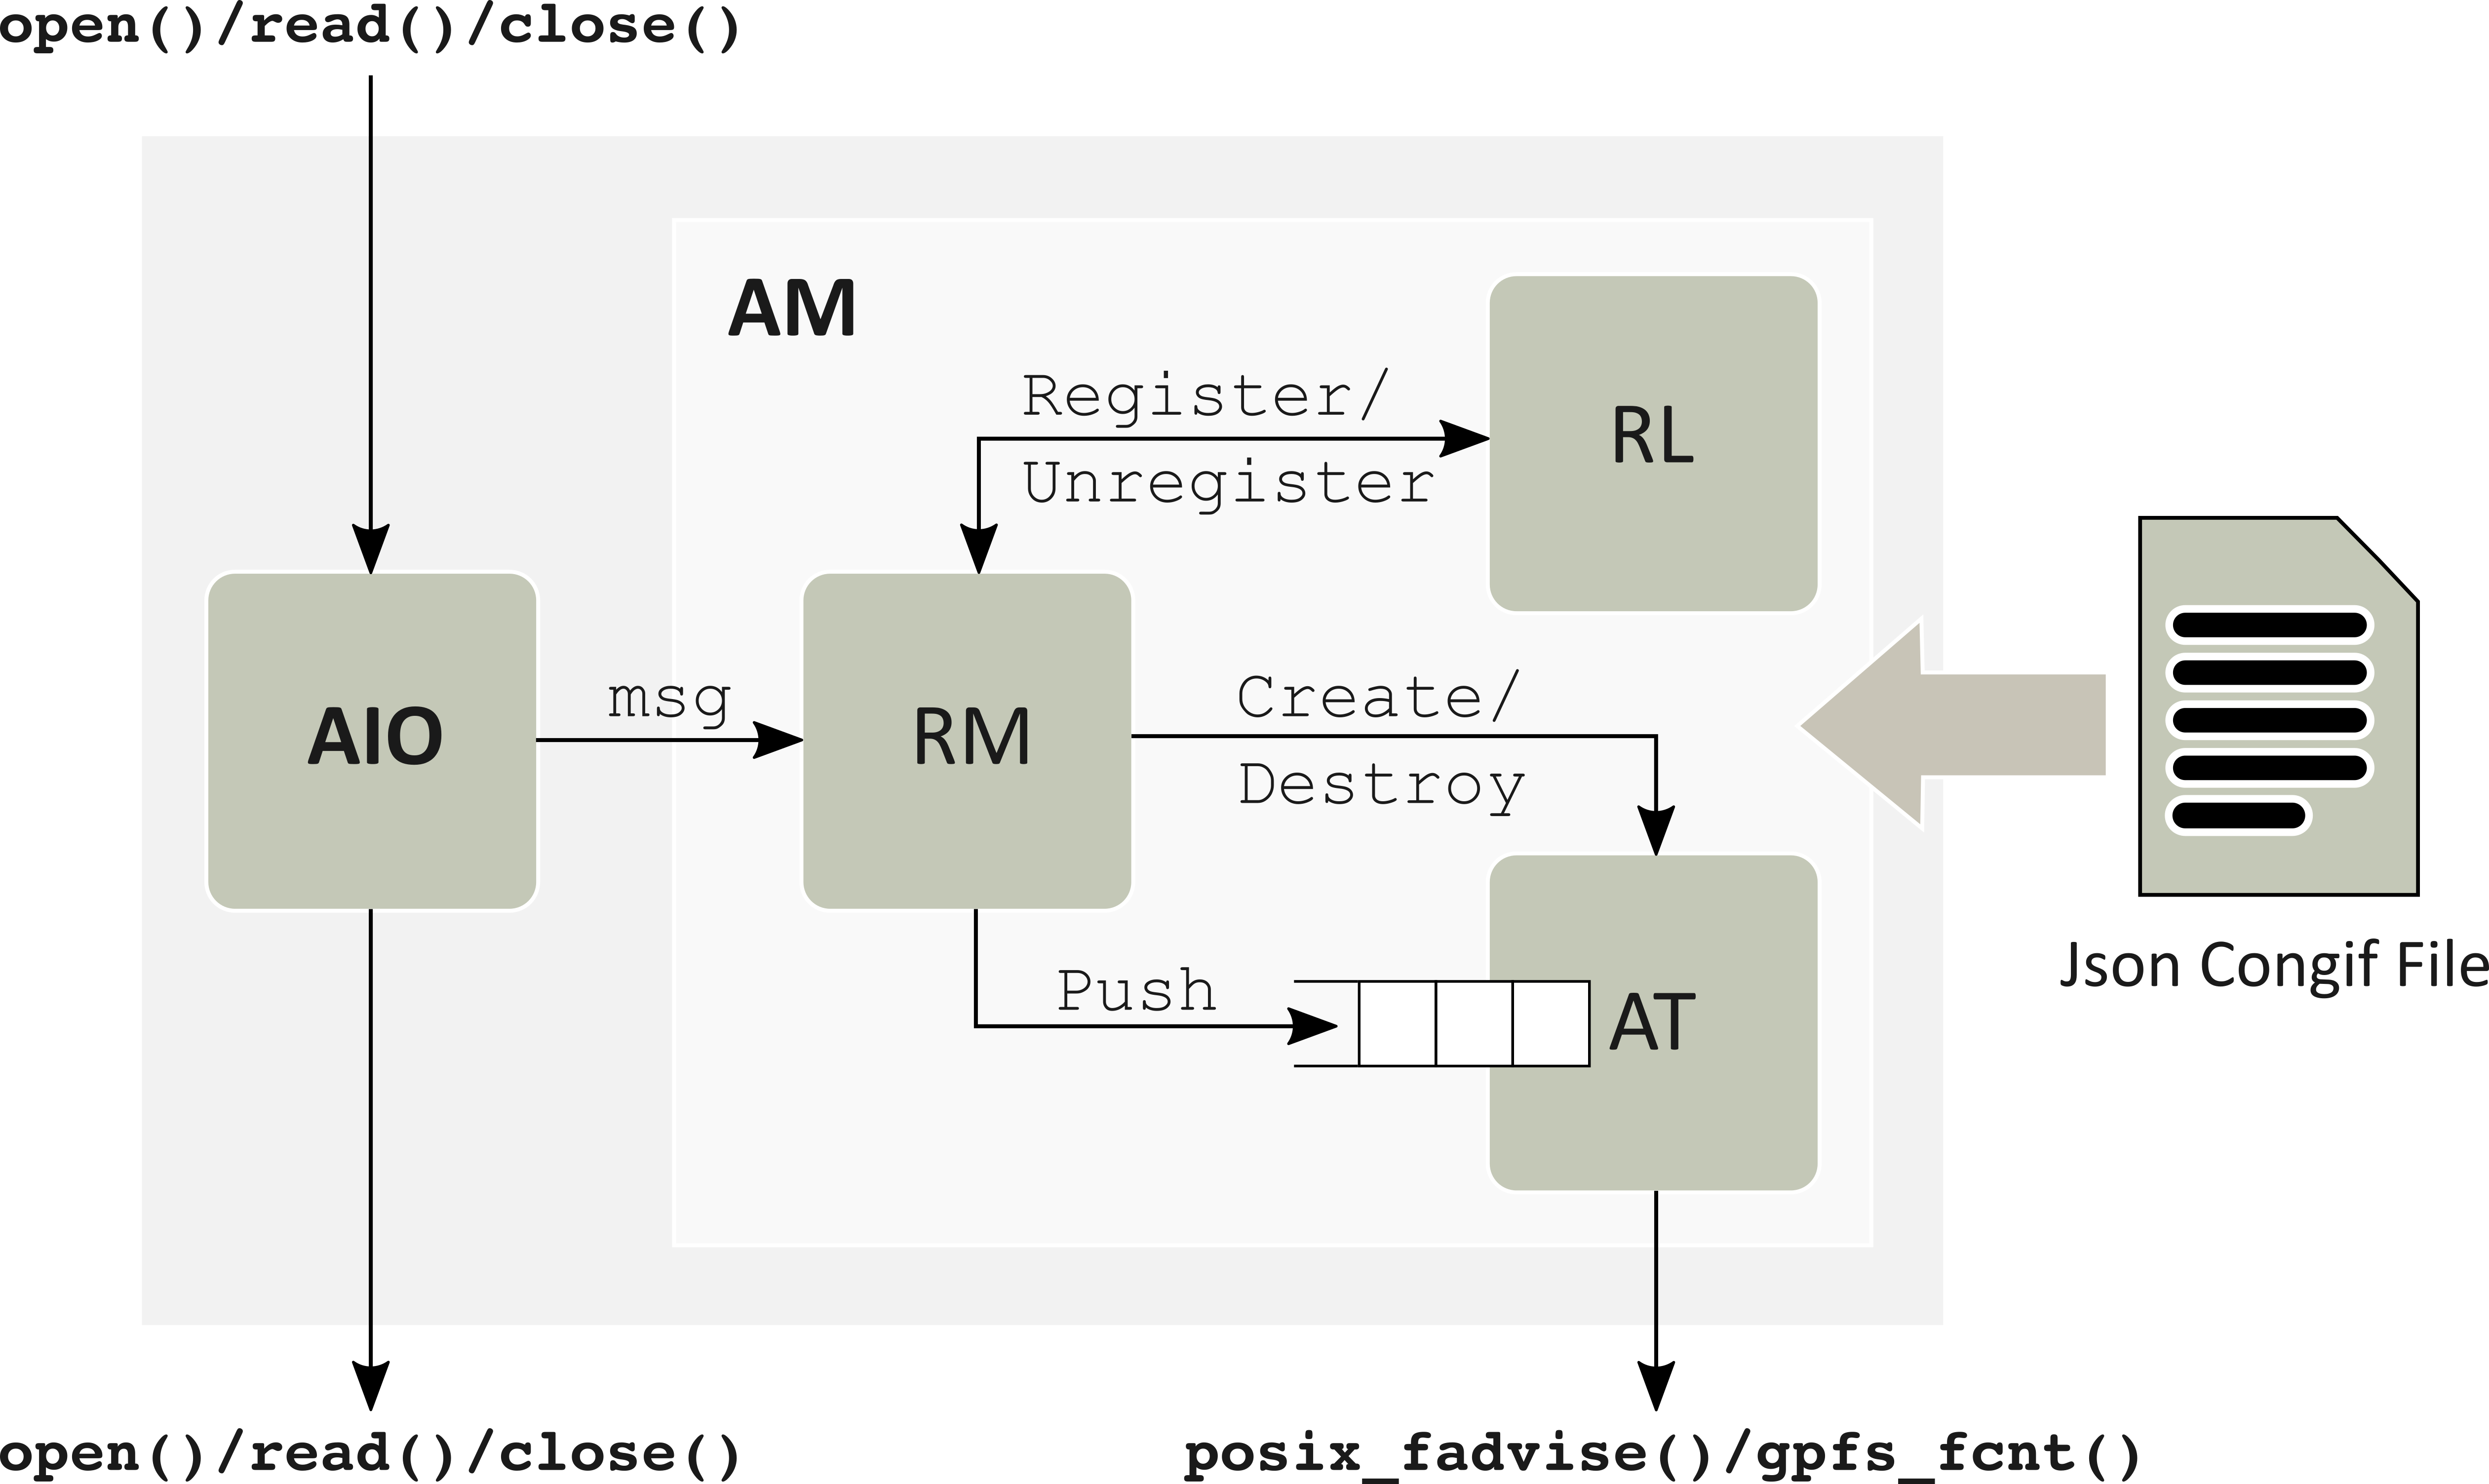
\includegraphics[width=0.8\textwidth]{chapters/chapter2/figures/mercury-architecture}
  \caption{Detailed architecture for the \textit{Advice Manager} (AM) component. This can be further divided into three blocks: \textit{Request Manager} (RM), \textit{Register Log} (RL), and \textit{Advisor Thread} (AT).}
  \label{figure: architecture}
\end{figure}

Both POSIX advice and GPFS hints affect an open file, identified by its file descriptor number. For the \textit{Advice Manager} to send advice or hints on behalf of the application, it needs to share the open file with the application. When sending messages from 
the \textit{Assisted I/O library} to the \textit{Advice Manager} we use \texttt{sendmsg()}. Besides normal data, this system call allows the transfer of ancillary (or control) information. One use of such information is to send a remote process a 
'file descriptor'~\cite{StevensR13} via a UNIX domain socket~\cite{UnixSock}. These numbers are just an index into the kernel's list of a process's open files. When sending a file descriptor using \texttt{sendmsg()}, the kernel copies a new reference to the open 
file descriptor, and adds it to the receiving process's open files list. The \textit{Advice Manager} receives a new file descriptor number, (which will likely be different to the number sent), which points to a file descriptor shared with the application. This 
allows us to send hints or advice for the shared file.

\subsection{File Data Prefetching}
\label{subsec: data_prefetching}
POSIX advice and GPFS hints are issued using the \textit{Advisor Thread} created by the \textit{Request Manager} during the register operation (Figure~\ref{figure: architecture}). When an application performs a read operation for an open file, the 
\textit{Assisted I/O library} sends to the \textit{Advice Manager} a message containing a string of the form: \texttt{"\textbf{Read} \textit{pid} \textit{fd} \textit{off} \textit{len}"}. This string includes the pid of the process, the application's file 
descriptor number for the file, the offset within the file and the length of the request. The pid and the file descriptor number are used by the \textit{Request Manager} module only to identify the corresponding \textit{Advisor Thread}. When the correct 
thread has been identified the \textit{Request Manager} pushes the offset and the length of the read request into a queue. This queue is accessed by the \textit{Advisor Thread} that uses the read information to trigger prefetch requests using the local file 
descriptor and keeps track of all the prefetched data using a block cache data structure. %Figure~\ref{figure: read_operation} shows the flow diagram for the read operation. 

The \textit{Advisor Thread} uses \texttt{posix\_fadvise()} and \texttt{gpfs\_fcntl()} to generate prefetch requests for the underlying file systems (Figure~\ref{figure: architecture}). For files residing in local file systems and Lustre, the 
\texttt{POSIX\_FADV\_WILLNEED} advice from Table~\ref{table: advice_table} is used to bring the data into the kernel page cache. For files residing in GPFS the \texttt{accRangeArray} in the \texttt{gpfsMultipleAccessRange\_t} data structure in Listing~\ref{list: mar} 
is used to define which blocks of the file should be brought into the GPFS internal cache (page pool). The size of the file regions to prefetch is defined in a Json\footnote{Open standard format that uses human-readable text to transmit data objects consisting 
of attribute-value pairs (http://www.rfc-editor.org/rfc/rfc7159.txt).} configuration file, loaded at startup by both the \textit{Advice Manager} and the \textit{Assisted I/O library}. This is the only point of configuration for the user and it contains, besides 
other information, a list of files and directories that the \textit{Assisted I/O library} should monitor. An example configuration file is shown below. 

\begin{lstlisting}[language=python, caption=Example of Json Configuration File, label={config}]
{
    "File": {
        "Path": "/path/to/target/file",
        "BlockSize": 4194304,
        "CacheSize": 8,
        "ReadAheadSize": 4,
        "WillNeed": {
            "Offset": 0,
            "Length": 0
        }
    },
    "Directory": {
        "Path": "/path/to/target/dir",
        "Random": {
            "Offset": 0,
            "Length": 0
        }
    }
}
\end{lstlisting}

As it can be seen in Listing~\ref{config} the structure of the configuration file is very simple. It allows users to define which files POSIX advice or GPFS hints should be applied to by setting the `Path' field to the full file path and the regions of the file 
that are likely to be accessed in terms of offset and length. In the case of POSIX advice users can also define directories to which a global advice should be applied (e.g. randomly accessed files in the directory). Additionally, when indicating a `WillNeed' 
advice users can directly control the caching behaviour of the \textit{Advisor Thread} block cache. In particular, they can define the granularity of the prefetch request (`BlockSize'), how many blocks can be fitted into the \textit{Advisor Thread} cache 
(`CacheSize') and how many blocks of data should be read ahead starting from the current accessed block (`ReadAheadSize'). Clearly the example in Listing~\ref{config} is not exhaustive. More complex configuration files can be generated by administrators 
(or automatic tools) to dynamically change the I/O patterns of applications in order to best adapt them to the underlying storage system.

The replacement policy for the block cache in the \textit{Advisor Thread} uses an LRU algorithm. In order to prefetch data, the open file is divided into blocks of size `BlockSize' and entire blocks are loaded/released into/from memory as the application 
progresses. In the case of GPFS the \texttt{accRangeArray} hint is used to prefetch up to `ReadAheadSize' blocks ahead starting from the block touched by the current request. When the number of blocks in the cache has reached `CacheSize', if more blocks are 
requested, older blocks will be released using the \texttt{relRangeArray} hint to make space for the new ones. In the case of POSIX advice, the behaviour is the same but blocks are loaded into memory using the \texttt{POSIX\_FADV\_WILLNEED} advice and released 
using the \texttt{POSIX\_FADV\_DONTNEED} advice. The hints interface is automatically selected by the \textit{Advice Manager} at runtime depending on the file system hosting the target file. 

The \textit{Advisor Thread} block cache also provides a very basic level of coordination among processes accessing the same file. In fact, different \textit{Advisor Thread} instances hinting the same file on behalf of different processes share the same block cache. 
Blocks requested by one process will appear in the block cache and future accesses to those blocks by other processes will not trigger new prefetching requests.

In general the configuration file can be used to describe any of the advice listed in Table~\ref{table: advice_table} and the hints listed in Table~\ref{table: hints_table}. To define a new scenario, we may consider a file region accessed sequentially for which 
the \texttt{POSIX\_FADV\_SEQUENTIAL} advice type could be used, and another region accessed randomly for which the \texttt{POSIX\_FADV\_RANDOM} advice type could be used. In this case, the configuration file would contain a list of file regions, specifying which 
type of advice messages are suitable. The right advice will be selected according to which part of the file is being accessed currently. This feature allows us to overcome another limitation of the Linux advice implementation that has been mentioned in 
Section~\ref{subsec: posix_advice_api}, namely, the first three advice types apply to the whole file since the implementation in the kernel completely disregards the byte ranges specified by the user.
 
Finally, when the application closes the file the \textit{Assisted I/O library} sends to the \textit{Advice Manager} a message containing a string of the form: \texttt{"\textbf{Unregister} \textit{pid} \textit{fd}"}. This string includes the pid of the process 
and the file descriptor number of the file to be closed. In response to this request the \textit{Request Manager} tells the \textit{Register Log} to unregister the file and destroys the \textit{Advisor Thread}, it also closes its shared copy of the file.

\subsection{POSIX Advice integration with Lustre}
\label{subsec: posix_advice_lustre}
Lustre is a high performance parallel file system for Linux clusters. It works in kernel space and takes advantage of the available page cache infrastructure. Additionally, it extends POSIX read and write operations with distributed locks to provide data 
consistency across the whole cluster. Even though Lustre makes use of the Linux kernel page cache, the previously described POSIX advice syscall has no effect on Lustre. The reason can be understood by looking at Figure~\ref{figure: kernel}. This reports the 
simplified call graph for the Lustre read operation in the file system client. To simplify the explanation, the figure is divided into four quadrants. Along the x-axis we have the native kernel functions (e.g. \texttt{generic\_file\_aio\_read}), separated by the 
Lustre specific functions (e.g. \texttt{lustre\_generic\_file\_read}). Along the y-axis we have page operations (e.g. \texttt{find\_get\_page}) separated by the file operations (e.g. \texttt{generic\_file\_aio\_read}). 

We can notice that Lustre extends the kernel code with additional file and page operations through the Lustre Lite component. These are the functions used by the kernel to fill the file operations table and the address space operations table. The 
\texttt{posix\_fadvise()} system call in the kernel translates into \texttt{fadvise64()}. In the case of \texttt{POSIX\_FADV\_WILLNEED} this function directly invokes \texttt{force\_page\_cache\_readahead()} which has no effect on 
\texttt{ll\_readpage()}. Other advice such as \texttt{POSIX\_FADV\_\{NORMAL,SEQUENTIAL,RANDOM\}} are disabled in Lustre by setting the kernel read-ahead window size to zero. This is done so that lustre will not speculatively try to gain a highly-contended 
lock to fulfil an optimistic read-ahead request.

\begin{figure}[!htb]
  \centering
  %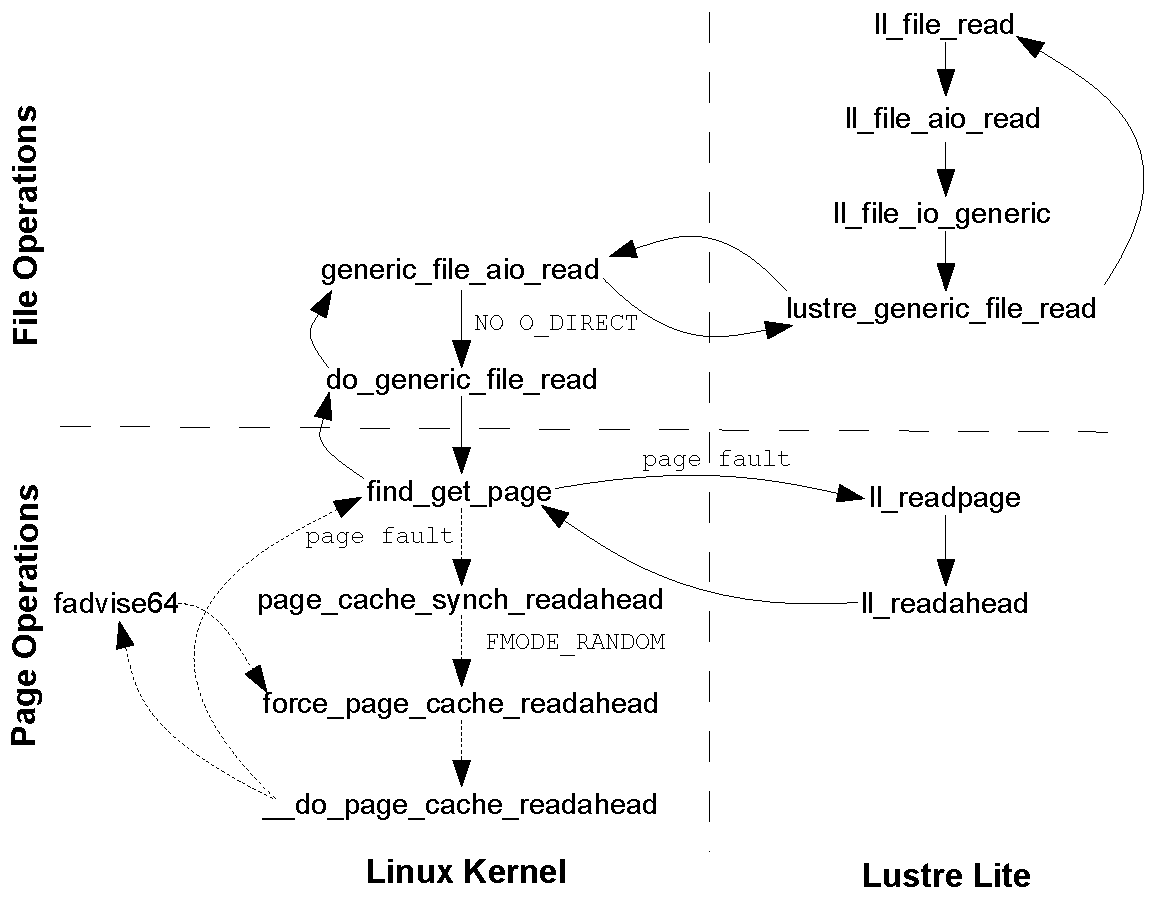
\includegraphics[width=0.8\textwidth]{chapters/chapter2/figures/kernel}
  \includegraphics[width=\textwidth]{chapters/chapter2/figures/linux_lustre_1}
  \caption{Simplified function call graph for the read operation in Lustre. For page operations in the Linux kernel the picture also shows the call graph typically followed by local reads as well as the call graph for the \texttt{POSIX\_FADV\_WILLNEED} advice in 
  the \texttt{posix\_fadvise()} implementation (dashed line).}
  \label{figure: kernel}
\end{figure}

In order to enable \texttt{POSIX\_FADV\_WILLNEED} in Lustre we modified the call graph of \texttt{fadvise64()} presented in Figure~\ref{figure: kernel} to invoke the \texttt{aio\_read()} operation in the file operations table for the open file and block until 
all the data has been read into the page cache. In this way we can force the kernel to invoke the corresponding file read operation in Lustre, acquiring locks as appropriate. Of course this mechanism still works with local file systems which eventually will end 
up calling \texttt{force\_page\_cache\_readahead()} as in the original version.

To prevent the new generated read from altering the read-ahead state of normal read operations, in \texttt{fadvise64()} we create a new \texttt{struct file} using the \texttt{dentry\_open()} routine and set the access mode flag (\texttt{f\_mode}) of the new file 
to \texttt{FMODE\_RANDOM} (which is exactly what the \texttt{POSIX\_FADV\_RANDOM} advice message does to disable read-ahead for random accessed files). This mechanism works perfectly with local file systems but has no effect on Lustre's read-ahead algorithm which 
is independent from the Linux kernel read-ahead. Therefore, \texttt{POSIX\_FADV\_WILLNEED} in the case of Lustre prefetches a bit more data than requested. This is acceptable for now but a future implementation will also modify the Lustre code to make sure the 
behaviour is the same in both cases.

Finally, our kernel patch does not require any user buffer to be provided with the new read operation. To avoid data being copied to user space we pass a null pointer to the \texttt{aio\_read()} routine. Additionally we defined a new \texttt{ki\_flag} for the 
kernel I/O control block (\texttt{kiocb}), that we called \texttt{KIF\_FORCE\_READ\_AHEAD}. This new flag is checked in the \texttt{generic\_file\_aio\_read()} routine and if set the \texttt{do\_generic\_file\_read()} routine is invoked with a pointer to the 
\texttt{file\_read\_actor\_dummy()} routine. \texttt{file\_read\_actor()} is normally the routine responsible for copying the data from the page cache to the user space buffer. Since in our case there is no user space buffer, the dummy routine just returns 
success.

\section{Evaluation}
\label{sec: mercury_evaluation}
We now present the evaluation of our \textit{Assisted I/O library} and \textit{Advice Manager} prototypes with a real world application used by physicists at the data processing center of the University of Mainz (ZDV). Our testbed is composed by 
a test cluster of seven nodes, mainly intended to evaluate the proposed Linux kernel modification with the Lustre file system. We start with a concise description of the system as well as a detailed analysis of the target application's I/O pattern, 
and then present the results of our experiments. 

We evaluate the performance of our framework using two metrics, the execution time of the test application and the number of reads completed by every target file system.

\subsection{Test Cluster}
\label{subsec: test_cluster}
As already mentioned, this small cluster is aimed mainly to test our modified kernel with Lustre. The reason is that it was not possible to disrupt the production cluster, affecting hundreds of users, by re-installing the operating system kernel. In order 
to make realistic comparisons between Lustre and GPFS, the test cluster also has a GPFS file system on comparable hardware. Both filesystems have a single disk server each, one Dell R710 acts as GPFS network shared disk (NSD) server and another as Lustre 
object storage server (OSS). The R710 are equipped with two quadcore E5620 @ 2.4 GHz and 24 GB main memory. For storage, both disk servers share a MD3200 array with 2 controllers and 4 MD1200 expansion shelves for a total of 60 2 TB drives. The Storage is 
formatted in 4 15 dynamic disk pools. This is the LSI/Netapp type of declustered RAID, which distributes the 8+2 RAID6 stripes evenly over all 15 disks for better rebuild performance. The disk block size is set to 128 KiB, which results in a RAID stripe size 
of 1MiB. The four disk pools are then split on the Array into LUNs, one of the LUNs from each disk pool is then used for GPFS and another one from each pool is used for Lustre. This results in comparable resources for both file systems and tests do not interfere 
with each other, as long as only one file system is tested at a time. While the GPFS file system embeds the metadata with the data, Lustre needs a separate Metadata Server (MDS). This is hosted by a SuperMicro server equipped with one quadcore Xeon E3-1230 
@3.3 GHz and 16 GB of main memory, as metadata target (MDT) it uses a 120 GB SSD Intel 520. Four other machines of the same type, equipped with an eight core E3-1230 @3.3 GHz processor and 16 GB of main memory, work as compute nodes and file system clients. 
All machines, servers and clients, are equipped with Intel X520DA 10 Gigabit adapters and connected to a SuperMicro SSE-X24S 24 ports 10 Gigabit switch. Both, the GPFS and Lustre file systems are formatted with a block size of 4 MB.

\subsection{Real World Application}
\label{subsec: application}
Our target real world application is written using `ROOT', an object-oriented framework widely adopted in the experimental high energy physics community to build software for data analysis. The application analyzes data read from an input file in the `ROOT' 
format (structured file format). 

\begin{figure*}[!htb]
  \centering
  \begin{subfigure}[t]{0.48\textwidth}
    \centering
    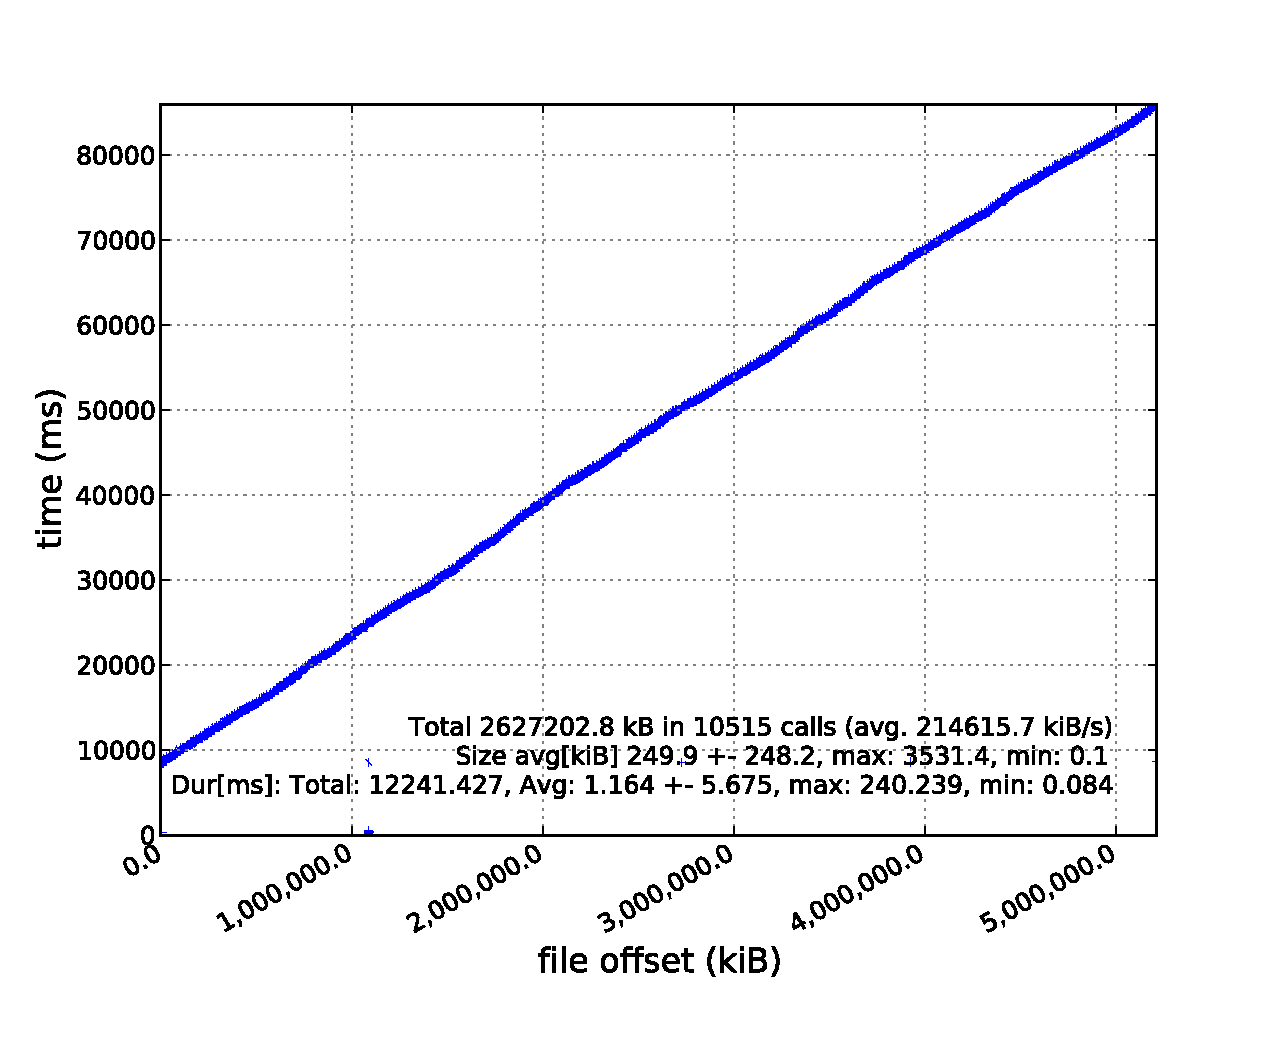
\includegraphics[width=\textwidth]{chapters/chapter2/figures/iopat_profile}
    \caption{\textit{}}
    \label{figure: iopat_profile}
  \end{subfigure}
  \begin{subfigure}[t]{0.48\textwidth}
    \centering
    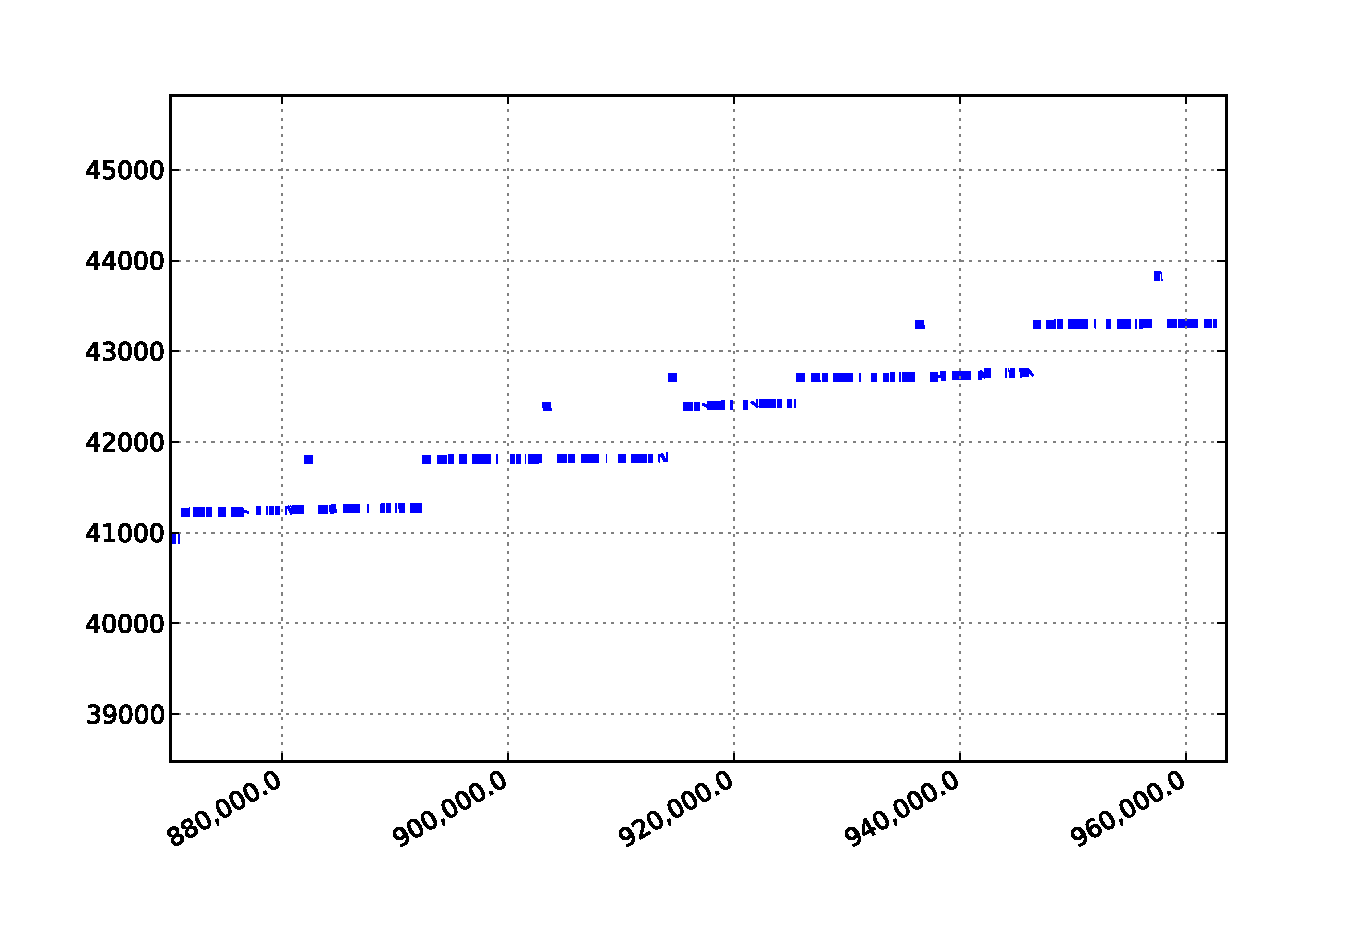
\includegraphics[width=\textwidth]{chapters/chapter2/figures/00050_zoom}
    \caption{\textit{}}
    \label{figure: iopat_zoom}
  \end{subfigure}
  \caption{I/O read profile of the target application under analysis (\ref{figure: iopat_profile}), extracted from the the GPFS file system in the test cluster, and zoomed window (\ref{figure: iopat_zoom}) showing the actual pattern details.}
  \label{figure: iopattern_with_statistics}
\end{figure*}

First of all we characterized the application's I/O pattern for a target file using traces and statistics extracted through several tools such as \textit{strace}, \textit{ioapps}~\cite{ioapps} and GPFS's \textit{mmpmon}~\cite{mmpmon} monitoring tool. 
Figure~\ref{figure: iopattern_with_statistics} shows the I/O pattern along with some additional statistics. As it can be seen, in this specific case (5 GB file), the application issues a total of 10515 \texttt{read()} system calls to read about 2.6 GB of 
total data. The average request size is 250 kiB and the time spent waiting for I/O is 12 seconds, when running on the test cluster. 

At a first glance the general I/O behaviour of the application looks linear, most of the accesses to the file follow an increasing offset. Nevertheless, adjacent reads are separated by gaps (a strided read pattern). In a few cases this gap becomes negative, 
meaning that the application is moving backwards in the file to read some data previously left behind (as reported in Figure~\ref{figure: iopat_zoom}).

After a detailed I/O pattern analysis we could divide the target file into contiguous non overlapping ranges. Within these ranges reads happen to have increasing offset. Even though the general I/O pattern of the application for different files looks similar
\footnote{Due to space limits we do not report the comparison between different files.}, the size of the non overlapping ranges may change significantly. This general behaviour can be modelled using a configuration file in which a `WillNeed' hint covers the 
whole file from beginning to end (i.e. `Offset' and `Length' equal to 0). The backwards seeks can be accounted for using the `CacheSize' parameter to keep previously accessed blocks in cache. In this way we effectively emulate a sliding window that tracks the 
application's I/O behaviour. This would not be possible by just using a, e.g., \texttt{POSIX\_FADV\_WILLNEED} advice on the whole file before starting the application like shown by Figure~\ref{figure: fadvise_comparison}. The reason is that if the file size 
is equal or smaller than the cache size, we would have a large number of valuable pages discarded from the cache to load data that will be accessed at the end of the application. Additionally, if the file size is bigger than the cache size we would have the 
file system discarding blocks at the beginning of the file as the blocks at the end are preloaded, effectively forcing the application to access these blocks from the I/O servers instead of the cache. With our approach, on the other hand, we keep in the cache 
only a small, controlled number of blocks (the ones currently accessed), while the older blocks are discarded since no longer needed. 

\begin{figure}[!htb]
  \centering
  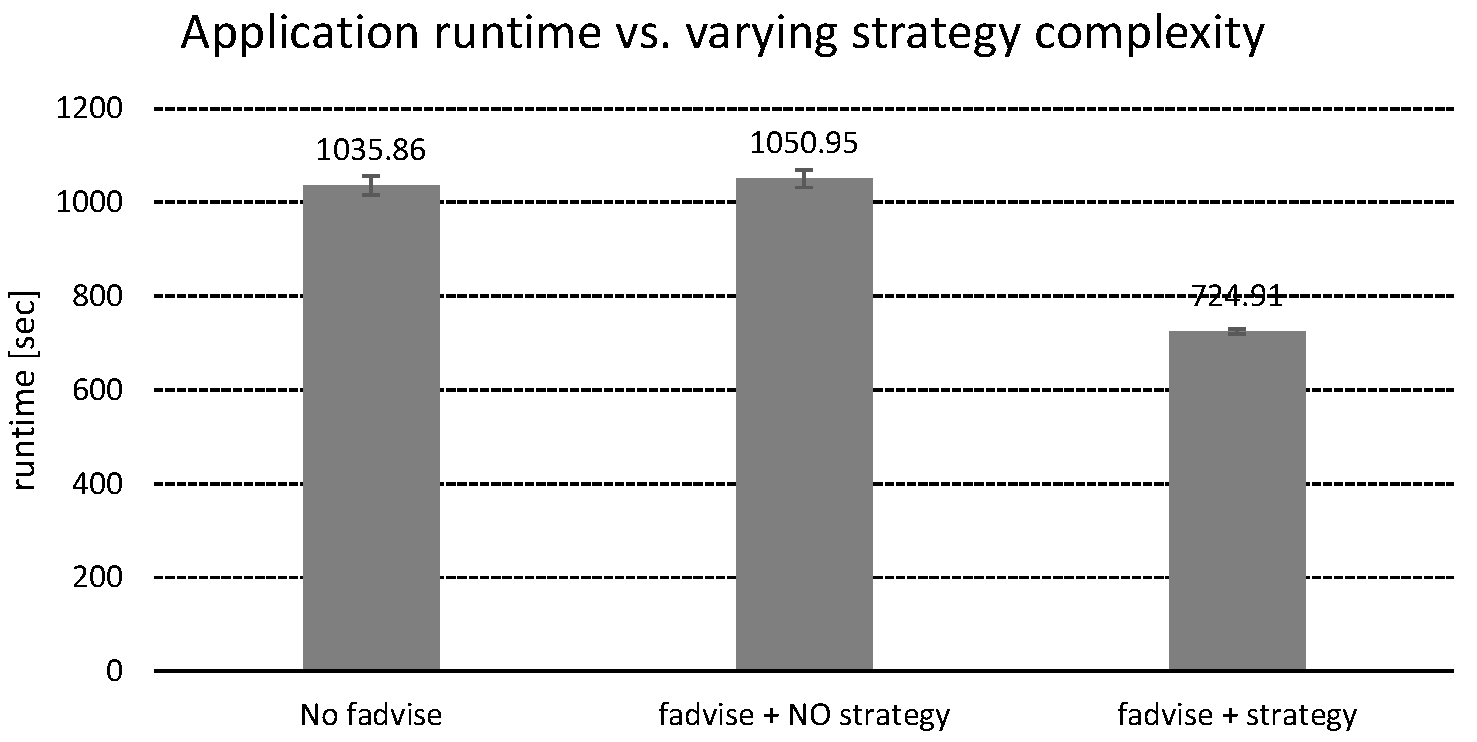
\includegraphics[width=0.8\textwidth]{chapters/chapter2/figures/SC2015/ROOT/separate_plots/test_cluster/test_fadvise_no_border}
  \caption{Comparison between different usage stategies of posix\_fadvise for an input file of 55 GB residing in an ext4 file system. The first bar represents the case in which no advice is used, the second bar represents the case in which a 
  POSIX\_FADV\_WILLNEED is issued for the whole file at the beginning of the application and the third bar represents the case in which POSIX\_FADV\_WILLNEED is issued using MERCURY.}
  \label{figure: fadvise_comparison}
\end{figure} 
 
To assess the impact of our prototype on the application and file systems performance we considered the application execution time and the number of reads accounted for by the respective file systems. We conducted our experiments without file system hints 
and then with file system hints issued transparently to the application by the \textit{Advice Manager}. Furthermore, we ran each experiment three times and calculated average, minima and maxima for each metric. In order to avoid caching affecting our 
measurements, extra care was taken to clean all the relevant caches for the different file systems. For ext4 and Lustre this was accomplished by using the command line: $$echo\ 3 > /proc/sys/vm/drop\_caches$$ on the file system clients. Additionally, 
for Lustre this command was also executed on the OSS to avoid the server side cache to be retained. In the case of GPFS, the file system client's page pool was cleaned using the clean file cache hint in Table~\ref{table: hints_table}, the NSD servers do 
not cache any data. 

\subsection{Execution Time}
\label{subsec: results}
To measure the performance improvements that our prototype can deliver to the application's runtime we conducted two set of tests. In the first test we varied the size of the input file from 5 to 95 GB. This is mainly aimed to study the behaviour of the 
`ROOT' application using different input file sizes and how our solution behaves when the file becomes bigger than the available cache space. In the second test we varied the number of `ROOT' instances running simultaneously from 1 to 8. By doing so we study 
the interaction of multiple processes accessing the file system and how these can benefit from the prefetching hints generated by MERCURY. Figure~\ref{figure: runtime} reports the results for the described experiments. All the tests where performed using 
a `BlockSize' of 4 MB, a `CacheSize' of 8 blocks, a `ReadAheadSize' of 4 blocks, and a `WillNeed' hint covering the whole file (i.e. with `Offset' and `Length' equal to 0), resulting in each process consuming up to 32 MB of cache space and 512 MB in total 
for 8 application instances. The `WillNeed' on the whole file causes the \textit{Advisor Thread} to issue up to 4 (`ReadAheadSize') prefetching requests for blocks of 4 MB sequentially, starting from the current accessed block. This has the same effect of 
data sieving in ROMIO, optimizing the access size and allowing the application to read the requested data randomly from the cache instead of the file system. The produced effect is particularly beneficial in the case of Lustre and ext4, as it can be seen 
in Figures~\ref{figure: ext4_1} and~\ref{figure: lustre_1}. In these cases we measure reductions in the execution time of up to 50\% circa, with respect to the normal case. For GPFS we can still observe an improvement but this is more contained compared 
to the other file systems (Figure~\ref{figure: gpfs_1}). The reductions in the execution time measured in GPFS are on average up to 10\%, with respect to the normal case. The reason is that the default prefetching strategy in GPFS works better that traditional 
read-ahead. In fact, by disabling the prefetching in GPFS we observed reductions in the execution time comparable to the other file systems (not reported here).

\begin{figure*}[!htb]
  \centering
  \begin{subfigure}[t]{0.32\textwidth}
    \centering
    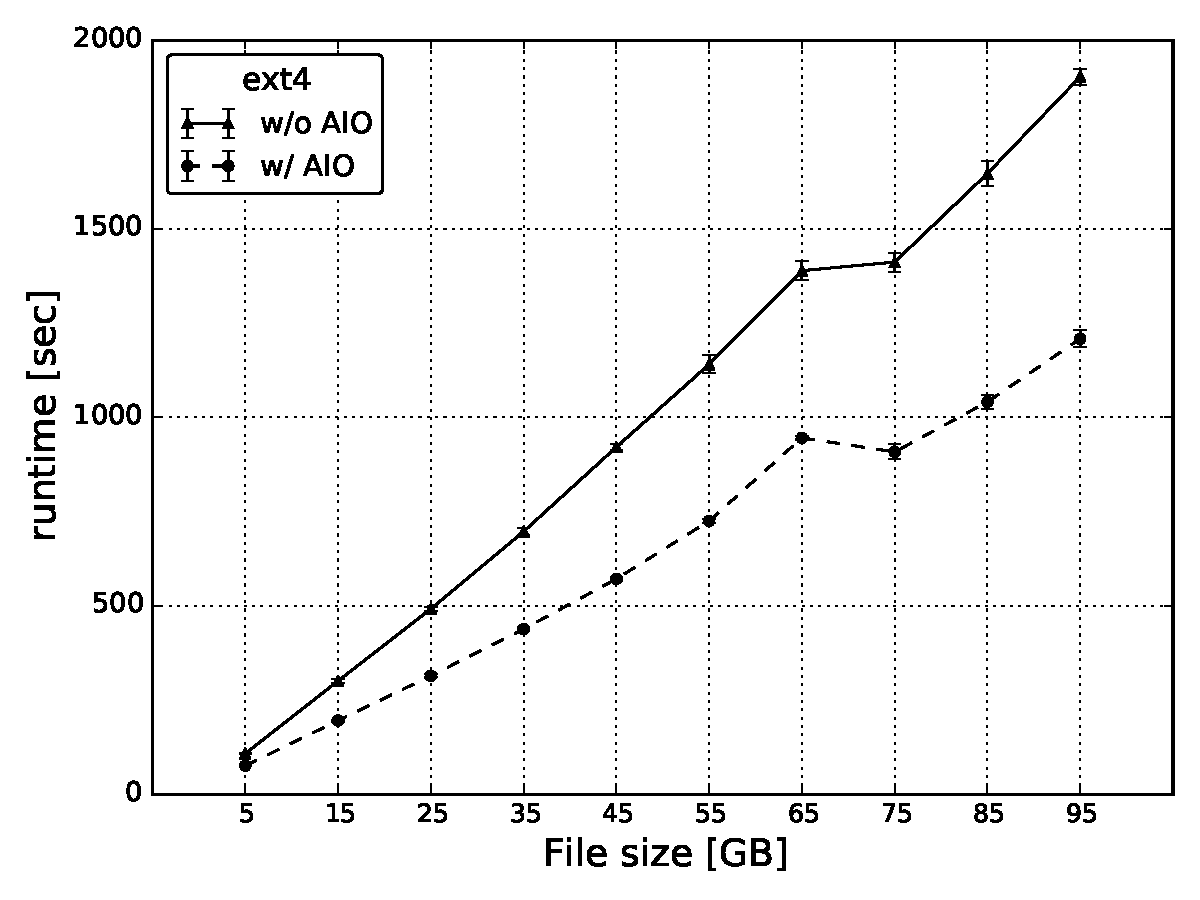
\includegraphics[width=\textwidth]{chapters/chapter2/figures/SC2015/ROOT/separate_plots/test_cluster/ext4/runtime}
    \caption{\textit{}}
    \label{figure: ext4_1}
  \end{subfigure}
  \begin{subfigure}[t]{0.32\textwidth}
    \centering
    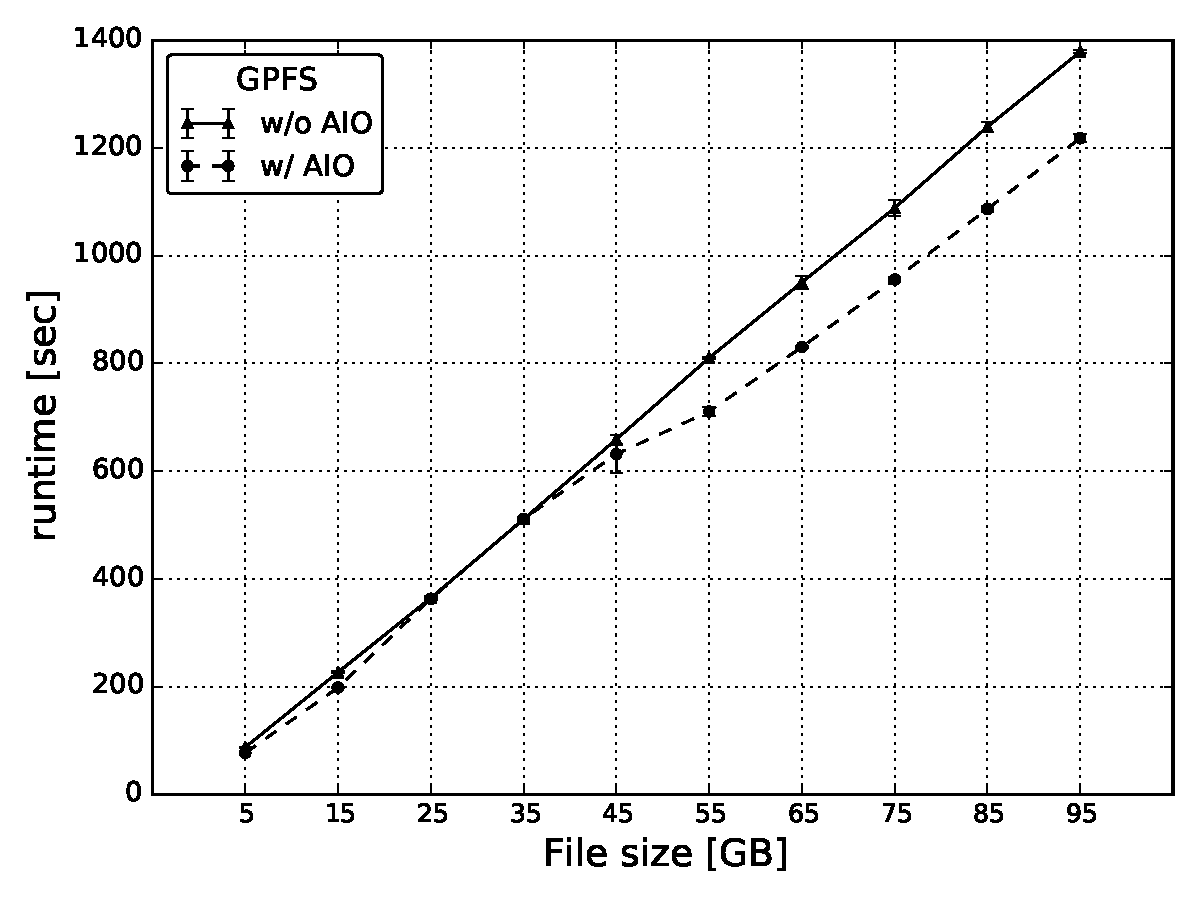
\includegraphics[width=\textwidth]{chapters/chapter2/figures/SC2015/ROOT/separate_plots/test_cluster/gpfs/runtime}
    \caption{\textit{}}
    \label{figure: gpfs_1}
  \end{subfigure}
  \begin{subfigure}[t]{0.32\textwidth}
    \centering
    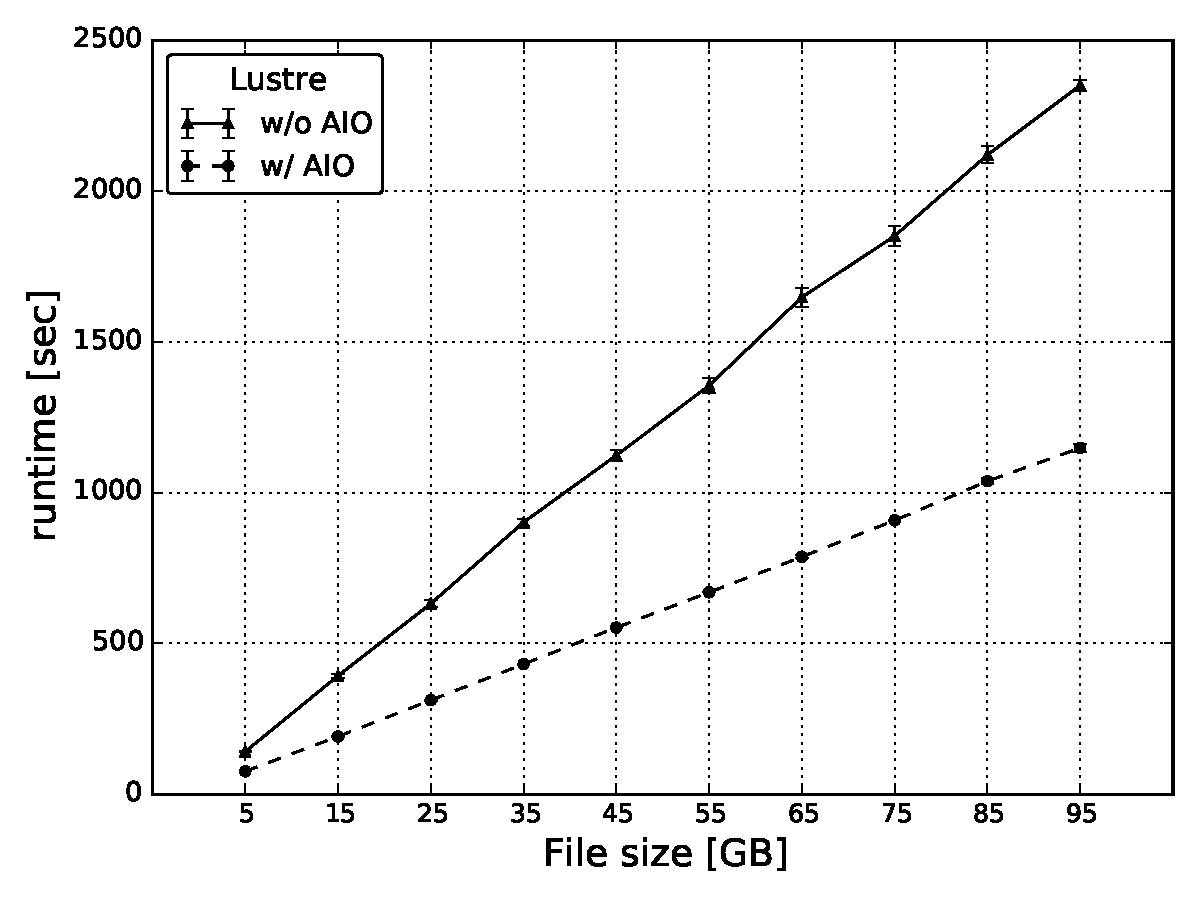
\includegraphics[width=\textwidth]{chapters/chapter2/figures/SC2015/ROOT/separate_plots/test_cluster/Lustre/runtime}
    \caption{\textit{}}
    \label{figure: lustre_1}
  \end{subfigure}
  \begin{subfigure}[b]{0.32\textwidth}
    \centering
    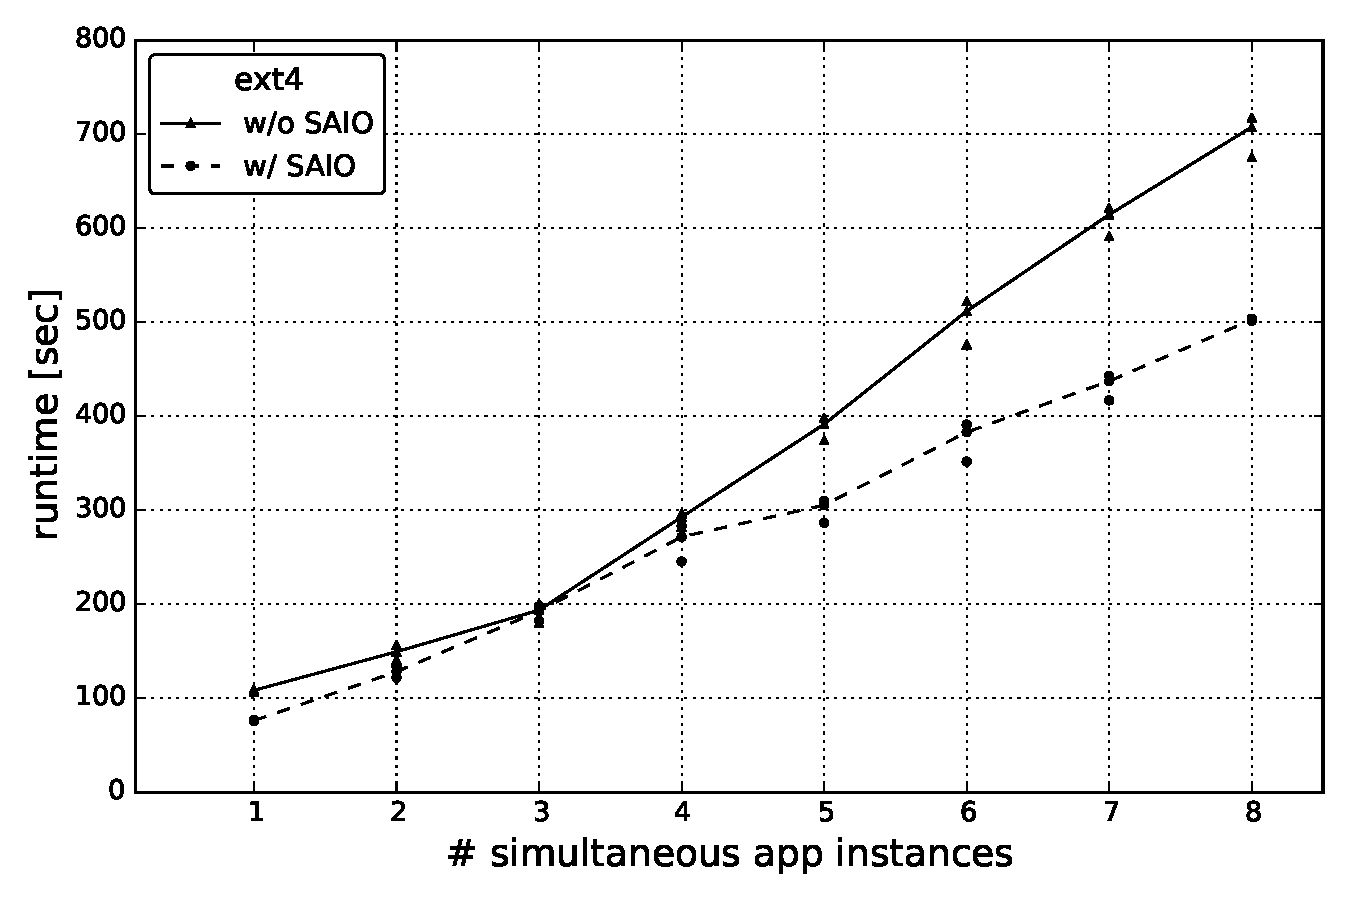
\includegraphics[width=\textwidth]{chapters/chapter2/figures/SC2015/ROOT/cluster/multiple_instances/simult_instance_ext4_test_cluster}
    \caption{\textit{}}
    \label{figure: ext4_2}
  \end{subfigure}
  \begin{subfigure}[b]{0.32\textwidth}
    \centering
    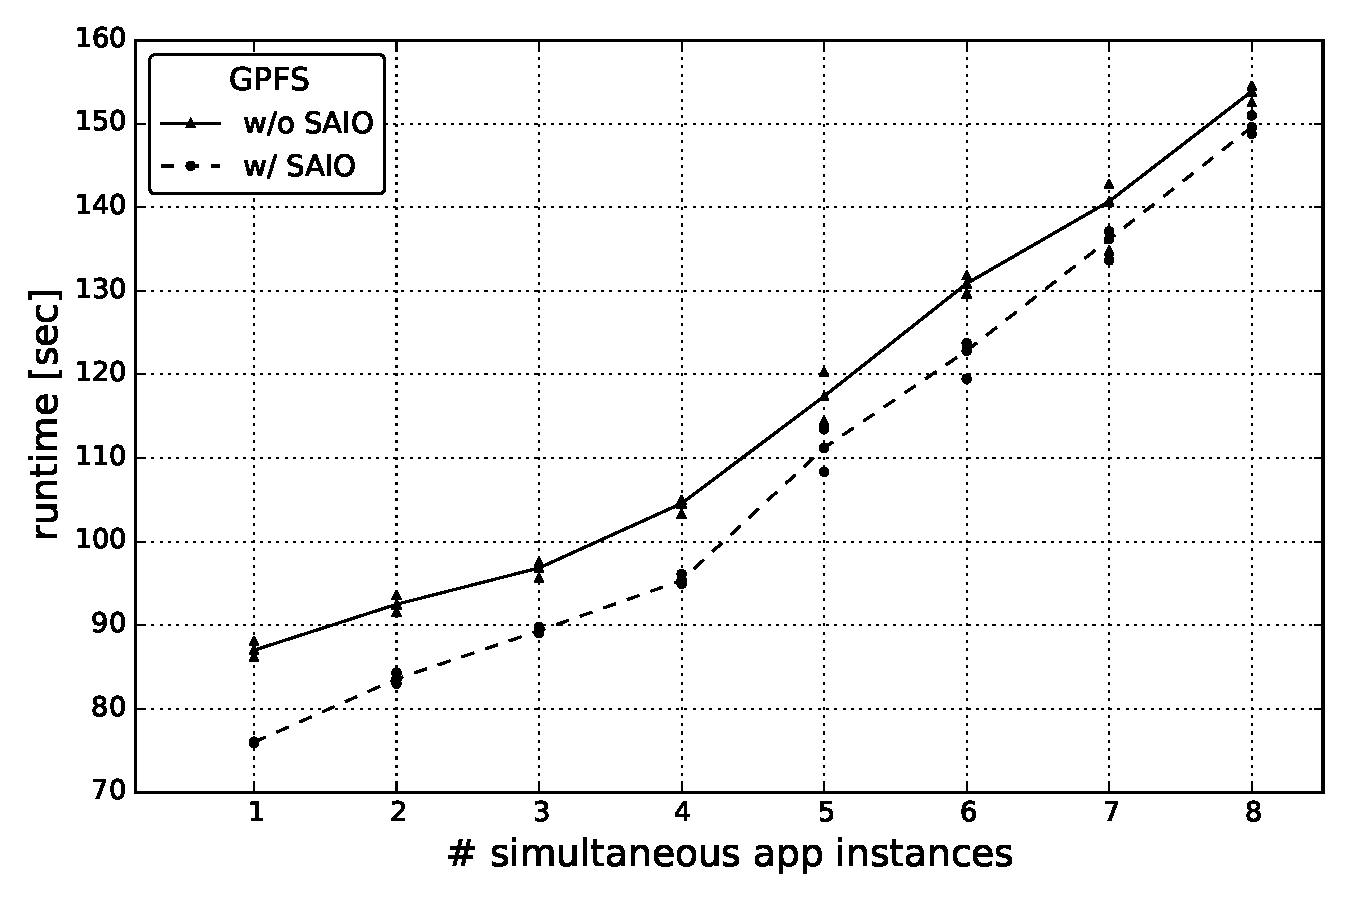
\includegraphics[width=\textwidth]{chapters/chapter2/figures/SC2015/ROOT/cluster/multiple_instances/simult_instance_gpfs_test_cluster}
    \caption{\textit{}}
    \label{figure: gpfs_2}
  \end{subfigure}
  \begin{subfigure}[b]{0.32\textwidth}
    \centering
    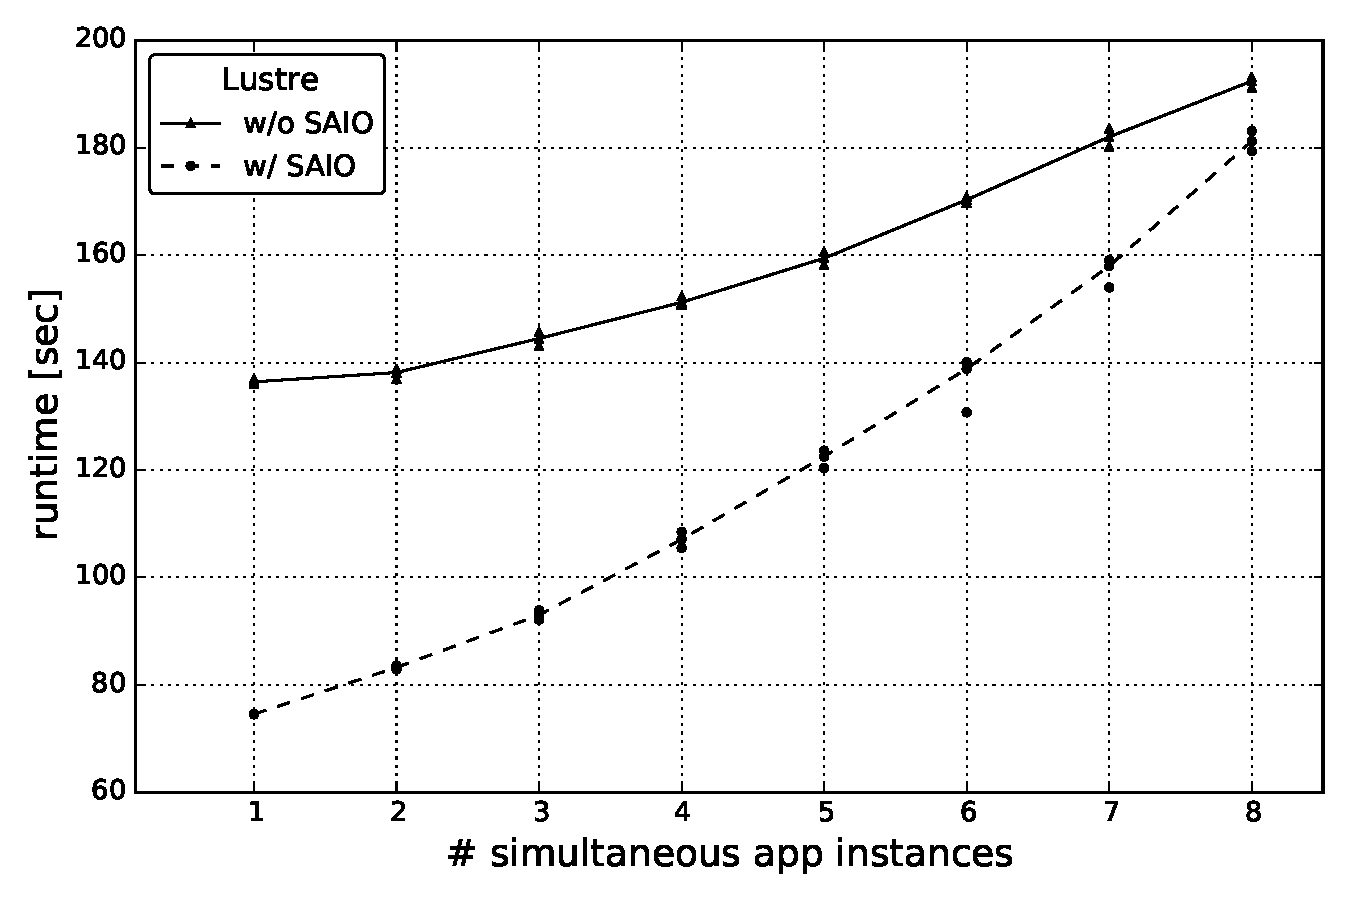
\includegraphics[width=\textwidth]{chapters/chapter2/figures/SC2015/ROOT/cluster/multiple_instances/multiple_simult_procs_Lustre_testcluster}
    \caption{\textit{}}
    \label{figure: lustre_2}
  \end{subfigure}
  \caption{Running time of the ROOT application for the three file system under study using different input file sizes (\ref{figure: ext4_1},~\ref{figure: gpfs_1} and~\ref{figure: lustre_1}) 
  and different number of instances accessing a file of 5 GB (\ref{figure: ext4_2},~\ref{figure: gpfs_2} and~\ref{figure: lustre_2}).}
  \label{figure: runtime}
\end{figure*}
\begin{figure*}[!htb]
  \centering
  \begin{subfigure}[t]{0.32\textwidth}
    \centering
    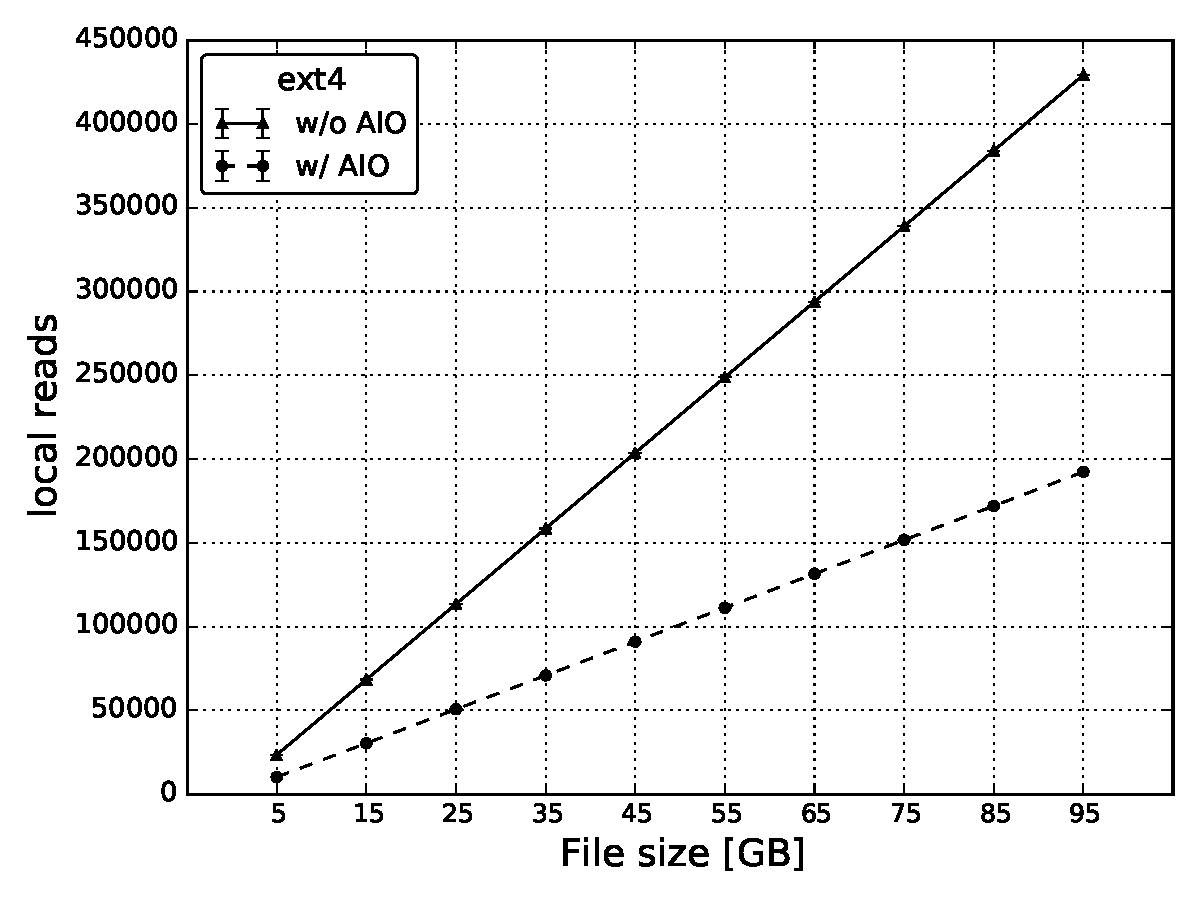
\includegraphics[width=\textwidth]{chapters/chapter2/figures/SC2015/ROOT/separate_plots/test_cluster/ext4/reads}
    \caption{\textit{}}
    \label{figure: ext4_3}
  \end{subfigure}
  \begin{subfigure}[t]{0.32\textwidth}
    \centering
    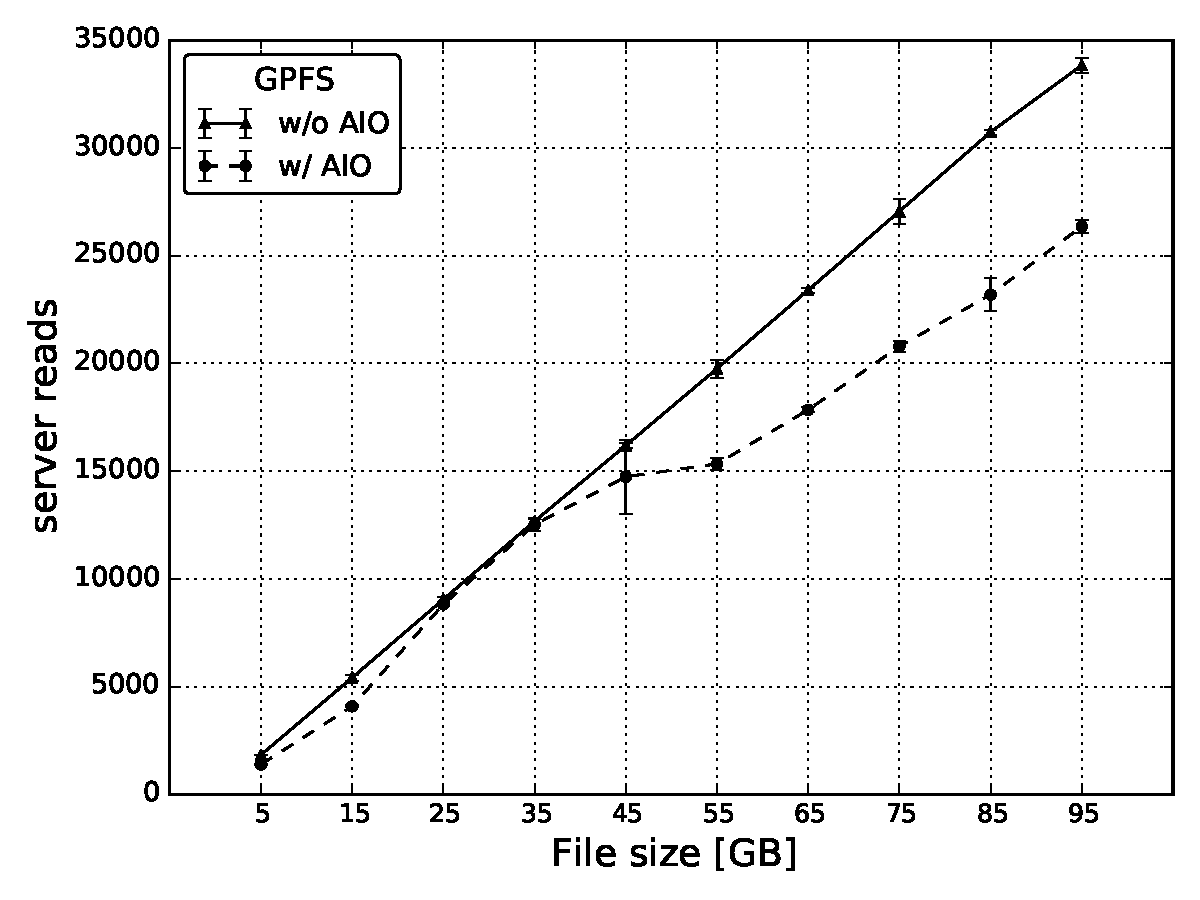
\includegraphics[width=\textwidth]{chapters/chapter2/figures/SC2015/ROOT/separate_plots/test_cluster/gpfs/server_reads}
    \caption{\textit{}}
    \label{figure: gpfs_3}
  \end{subfigure}
  \begin{subfigure}[t]{0.32\textwidth}
    \centering
    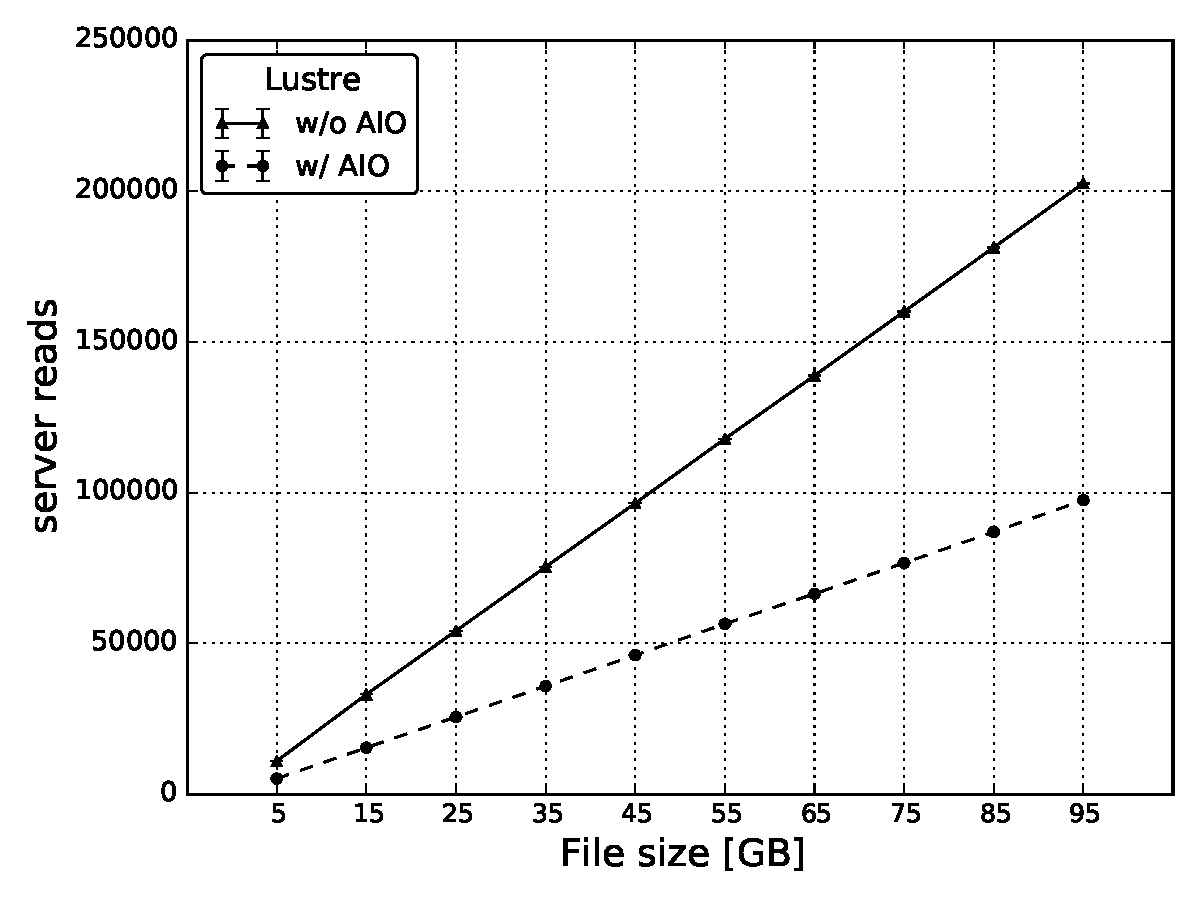
\includegraphics[width=\textwidth]{chapters/chapter2/figures/SC2015/ROOT/separate_plots/test_cluster/Lustre/server_reads}
    \caption{\textit{}}
    \label{figure: lustre_3}
  \end{subfigure}
  \begin{subfigure}[b]{0.32\textwidth}
    \centering
    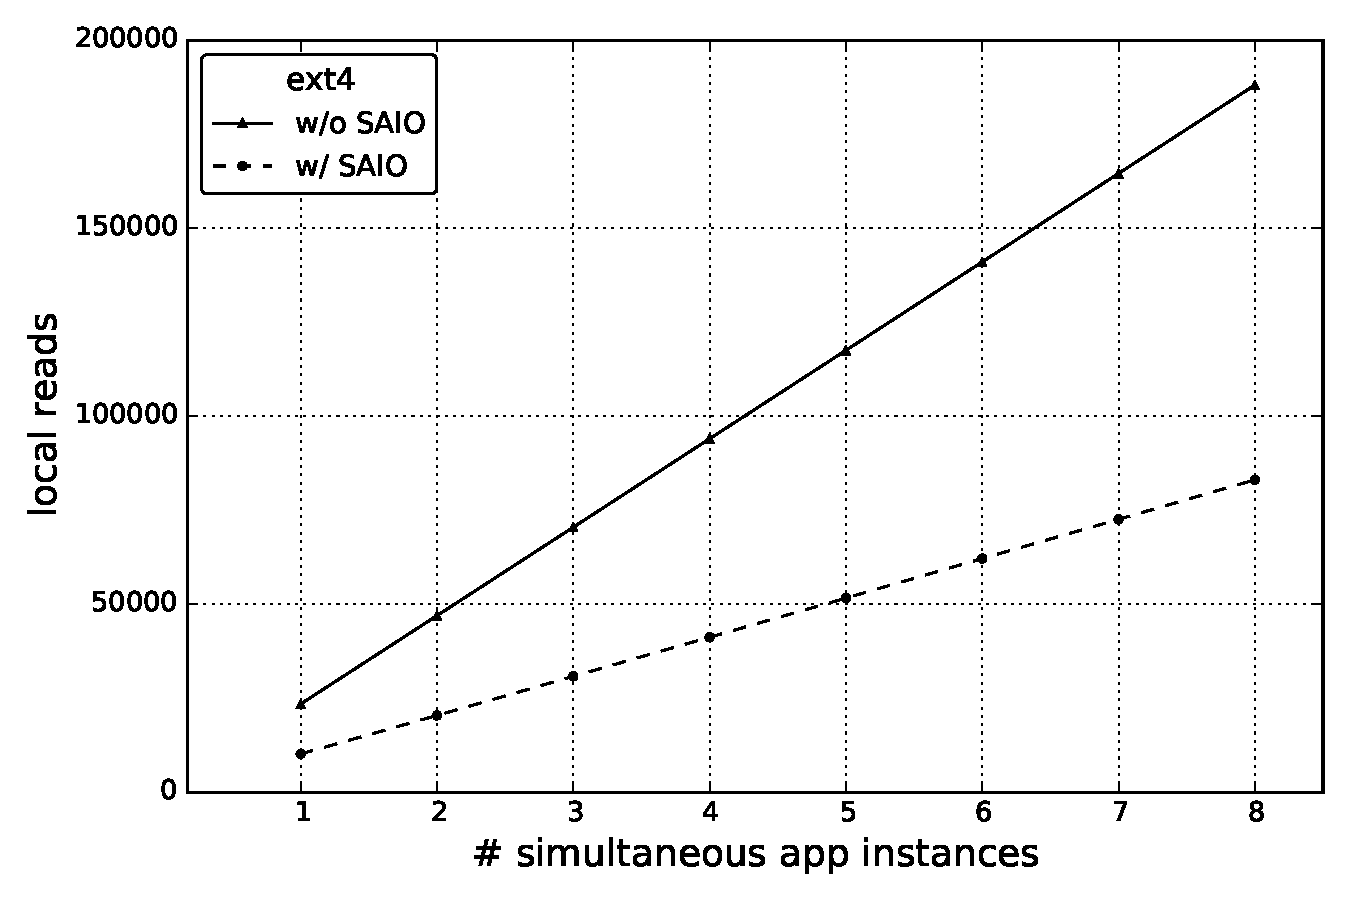
\includegraphics[width=\textwidth]{chapters/chapter2/figures/SC2015/ROOT/cluster/multiple_instances/reads_simult_instance_ext4_test_cluster}
    \caption{\textit{}}
    \label{figure: ext4_4}
  \end{subfigure}
  \begin{subfigure}[b]{0.32\textwidth}
    \centering
    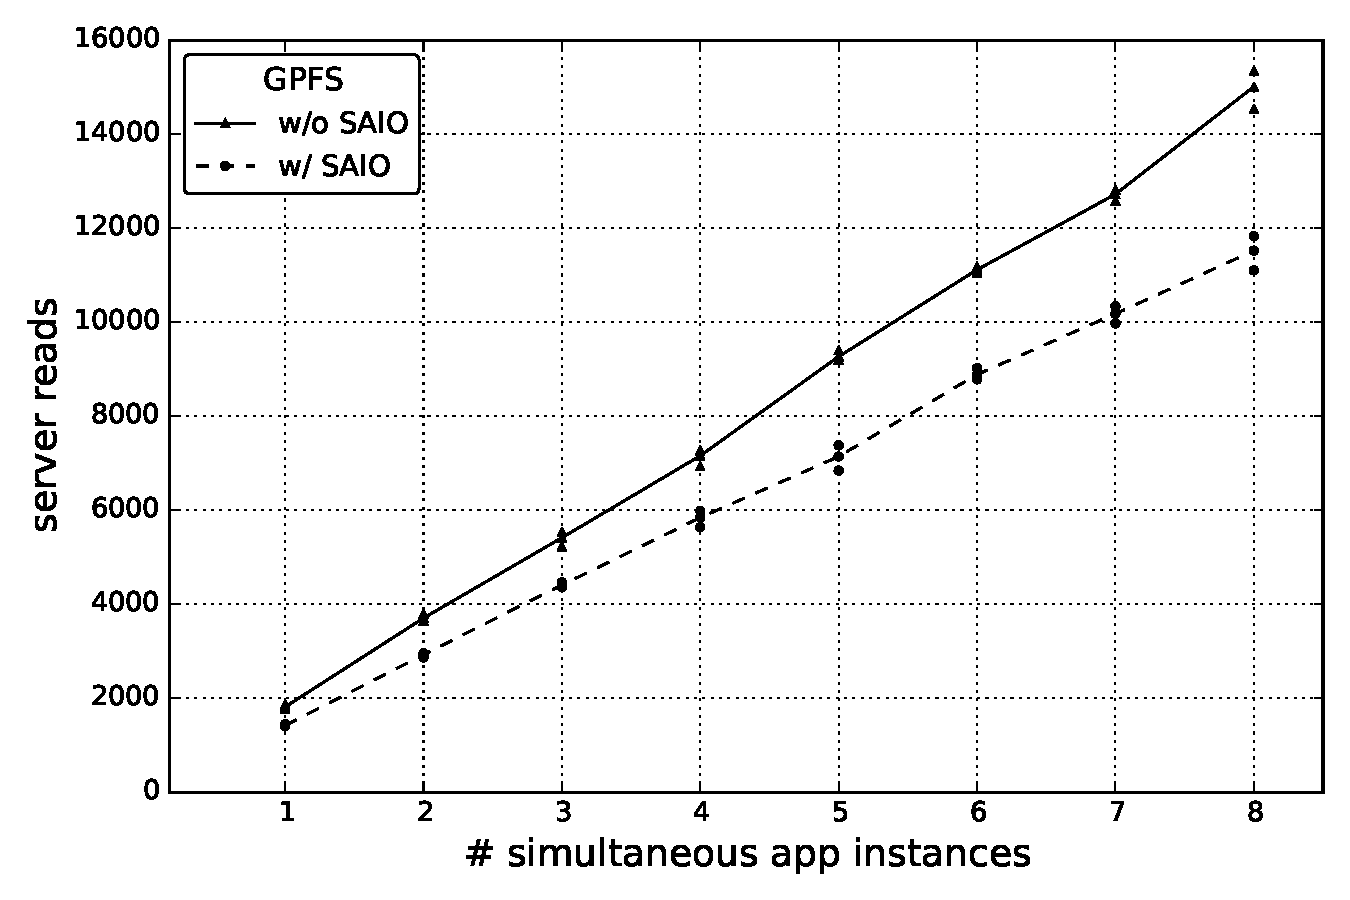
\includegraphics[width=\textwidth]{chapters/chapter2/figures/SC2015/ROOT/cluster/multiple_instances/reads_simult_instance_gpfs_test_cluster}
    \caption{\textit{}}
    \label{figure: gpfs_4}
  \end{subfigure}
  \begin{subfigure}[b]{0.32\textwidth}
    \centering
    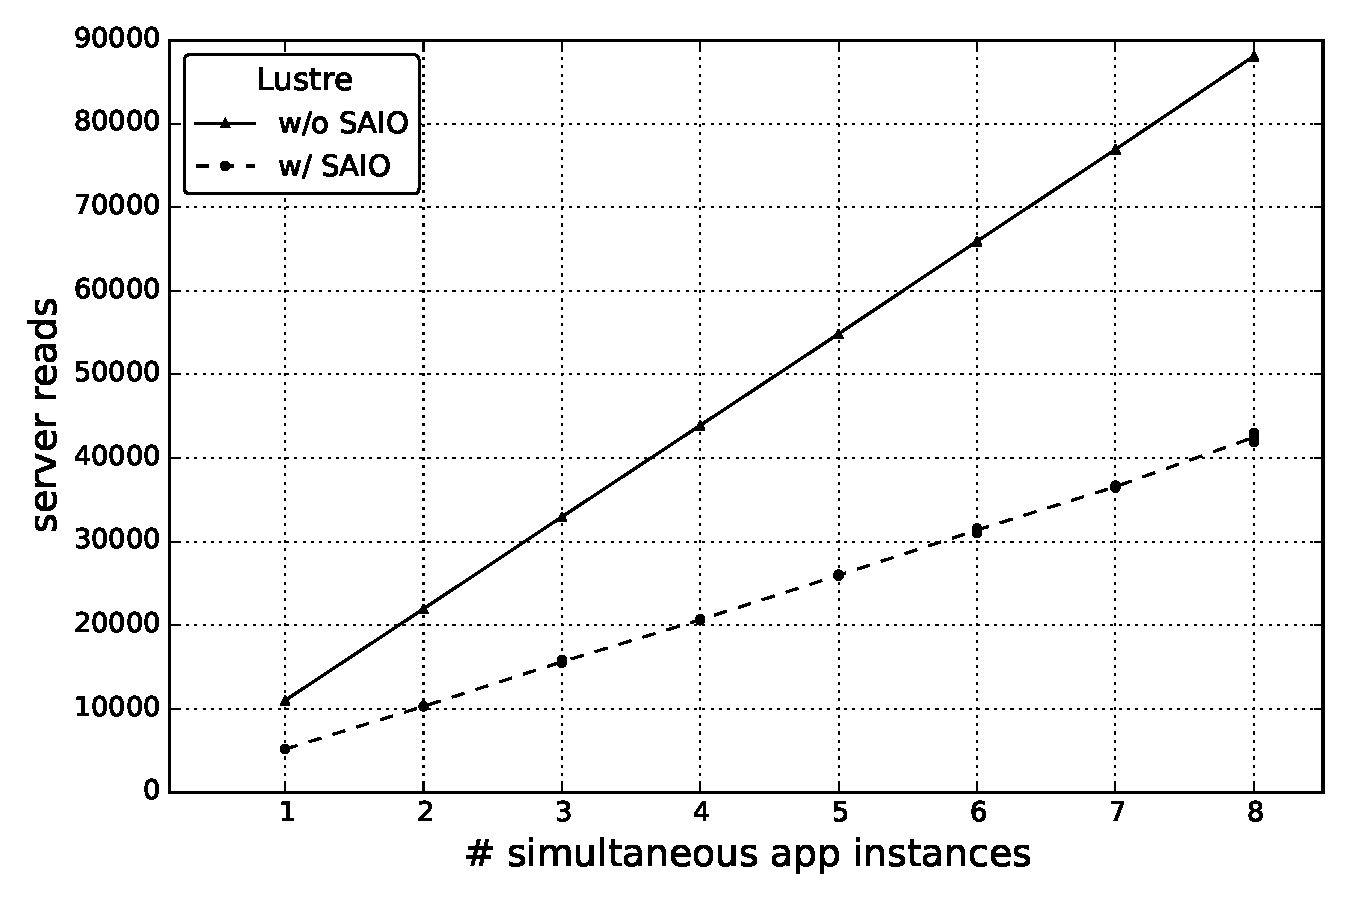
\includegraphics[width=\textwidth]{chapters/chapter2/figures/SC2015/ROOT/cluster/multiple_instances/reads_multiple_simult_procs_Lustre_testcluster}
    \caption{\textit{}}
    \label{figure: lustre_4}
  \end{subfigure}
  \caption{Reads processed by local ext4, GPFS and Lustre I/O servers for various input file sizes (\ref{figure: ext4_3},~\ref{figure: gpfs_3} and~\ref{figure: lustre_3}) and multiple instances of ROOT accessing a file of 5 GB (\ref{figure: ext4_4},
  ~\ref{figure: gpfs_4} and~\ref{figure: lustre_4}).}
  \label{figure: read}
\end{figure*}

As far as Figures~\ref{figure: ext4_2},~\ref{figure: gpfs_2} and~\ref{figure: lustre_2} are concerned, these account for the effect of processes' concurrency on the file system. Before continuing with the discussion we have to make a note here. 
In our architecture, only one process per file system's client issues (through multiple \textit{Advisor Thread}s) hints on behalf of running applications. This introduces some overhead, since we have to pass the access information from the 
\textit{Assisted I/O library} to the \textit{Advice Manager}, but has the advantage of better coordinating accesses to the same file from multiple processes. Nevertheless, we found that in the case of GPFS, despite the fact of having multiple 
\textit{Advisor Thread}s, only one process among the many was receiving a benefit from the prefetching hints. The reason is that GPFS seems to have the restriction of hinting only one file per process. For this reason, we developed another variant 
of Mercury in which the AIO library, now renamed \textit{Self Assisted I/O library} (SAIO), internally provides the creation and the handling of multiple \textit{Advisor Thread}s. Looking at the figures generated with the new SAIO library we can 
assess the effectiveness of the prefetching hints for the three file systems considered. In particular, Lustre provides the best runtime improvements compared to the case in which no hints were used. GPFS shows a more contained improvement since the 
I/O time is already small compared to Lustre and ext4. Finally, ext4 can really benefit from prefetching hints especially for high process counts. Overall, excluding ext4, when we increase the number of processes the runtime improvements shrink. This 
is probably due to the saturation of the file system client bandwidth.

\subsection{Read Request Rate}
\label{subsec: reads}
Figure~\ref{figure: ext4_3},~\ref{figure: gpfs_3} and~\ref{figure: lustre_3} report the number of read requests accounted for by the different file systems under study. In the specific, the figures show how the number of reads at the I/O server side 
for both GPFS and Lustre can be substantially reduced with our approach. This has a significant impact in HPC cluster in which the file system may be accessed by many thousand of processes at the same time. Reducing the number of requests for an application 
can increase the number of IOPS available for others. This result is also confirmed for multiple instances of the `ROOT' application running concurrently (Figure~\ref{figure: ext4_4},~\ref{figure: gpfs_4} and~\ref{figure: lustre_4}).

\section{Related Work}
\label{sec: mercury_related_work}
In the past researchers have tried to alleviate the I/O performance gap problem by analyzing I/O patterns and exploiting their knowledge to guide I/O using, for example, data prefetching. Tran and Reed~\cite{TranR04} presented an automatic time series 
modelling and prediction framework for adaptive I/O prefetching, named TsModeler. They combined ARIMA and Markov models to describe temporal and spatial behaviour of I/O patterns at file block level. TsModeler was integrated with the experimental file 
system PPFS2 to predict future accesses and tested against a selected physics code. Several characteristics, such as execution time improvements and cache miss reduction over different hardware configurations, are considered in the experiments. The results 
show that execution time can be reduced by the 30\% in some cases and cache misses can be reduced up to three order of magnitude. 
He et al.~\cite{HEBTAGGMCS13} proposed a pattern detection algorithm, based on the sliding window algorithm in LZ77 as base for building Markov models of I/O patterns at file block level. The model was afterwards used by a FUSE based file system to carry 
out prefetching. Chang and Gibson~\cite{ChangG99}, unlike previous works, did not build mathematical models but instead used speculative execution of the application code to guide data prefetching.

Other works tried to bring the same idea to higher level I/O libraries such as MPI I/O, HDF5 or PnetCDF to take advantage of the richer semantic, data dependencies and layout information. Chen, Byna, Sun, Thakur and Gropp~\cite{ChenBSTG08} proposed a 
pre-execution based prefetching approach to mask I/O latency. They provided every MPI process with a thread that runs in parallel and takes responsibility for prefetching future required data. Prefetching in the parallel thread was enabled via speculative 
execution of the main process code. Results, with PBench running on top of NFS and PVFS as file systems backend, show execution time reduction and sustained bandwidth improvements.
The same authors in~\cite{BynaCST08} proposed to exploit parallel prefetching using a client-side, thread based, collective prefetching cache layer for MPI I/O. The cache layer used I/O pattern information, in the form of I/O signatures, together with run 
time I/O information to predict future accesses. Experimental results show sustained bandwidth improvements even in this case. 
Chen and Roth~\cite{ChenR10} took inspiration from the collective I/O optimization enabled by ROMIO to design a collective I/O data prefetching mechanism that exploited global I/O knowledge. They compare the sustained bandwidth speed-up of individual 
prefetching with collective prefetching for a parallel benchmarking tool using PVFS2, and demonstrate that the latter performs better than the former by over two fold on average. 
He, Sun and Thakur~\cite{HEST12} proposed to analyze high level data dependencies exposed in PnetCDF, accumulate this knowledge building data dependency graphs and finally use them to perform prefetching. 

VanDeBogart, Frost and Kohler have previously used the Linux advice API to build a prefetching library~\cite{VanDeBogartFK09} for programmers to use. Prost et al. integrated the GPFS hint functionalities in the ROMIO ADIO driver for GPFS~\cite{ProstTHJK01}. 
In this context they exploit data type semantic in file views to prefetch parts of the file that will be soon accessed. 

In contrast to previous works, we do the following things differently. We do not try to automatically build mathematical models of I/O patterns and use them to accurately generate prefetching requests nor do we speculatively execute the application binary. 
In fact, we believe that users and administrators have the best understanding about the applications and their systems, and can exploit their knowledge and expertise to improve the storage system performance. We demonstrate that experienced users with a deep 
knowledge of their applications I/O behavior can convert non-optimal I/O patterns, in particular small random reads, into patterns that can be adapted to the underlying file system characteristics, and therefore give optimal performance. %In this work we focus on providing the infrastructure that enables users to access file system specific interfaces for guided I/O without modifying applications and hiding the intrinsic complexity that such interfaces introduce.  %and Indeed, we found that some I/O patterns look sequential if we observe them at a granularity coarser than the single request. 
Furthermore, previously described approaches are not suitable for small random read patterns since they rely on accurate knowledge of I/O behaviour % and the assumption that this remains unchanged over multiple runs of the application. Moreover, even if I/O patterns remain unchanged, the prefetching of random requests will still degrade the performance of the storage subsystem. 
to prefetch every single request one after the other. This still degrades the storage system performance due to the large number of I/O requests and seek operations hitting the storage devices. On the other hand, by using the POSIX advice and GPFS hints APIs, 
we can prefetch the region of the file that will be accessed and filter random requests using the cache. %Data prefetching allows us to increase the I/O bandwidth, reduce the number of I/O requests reaching the back-end storage devices and the execution time of applications. 

In this work we focus on providing the infrastructure that enables users to access file system specific interfaces for guided I/O without modifying applications and hiding the intrinsic complexity that such interfaces introduce. 
%.In this work we focus our attention on applications that use the POSIX I/O interface and have no access to the optimizations enabled by MPI I/O. Our idea is to exploit post morten I/O pattern analysis to generate advice and hints transparently for every file. 
